\documentclass[10pt,a4paper]{article}
\usepackage[latin1]{inputenc}
\usepackage[english]{babel}
\usepackage{amsmath}
\usepackage{amsfonts}
\usepackage{amssymb}
\usepackage{blkarray}
\usepackage{graphicx}
\usepackage{caption}
\usepackage{subcaption}
\usepackage{appendix}
\usepackage{listings}
\usepackage{biblatex}
\usepackage{hyperref}
\bibliography{refs.bib}
\usepackage{color}
\definecolor{dkgreen}{rgb}{0,0.6,0}
\definecolor{gray}{rgb}{0.5,0.5,0.5}
\definecolor{mauve}{rgb}{0.58,0,0.82}

\newenvironment{changemargin}[3]{%
\begin{list}{}{%
\setlength{\topsep}{0pt}%
\setlength{\leftmargin}{#1}%
\setlength{\rightmargin}{#1}%
\addtolength{\topmargin}{#2}
\addtolength{\textheight}{#3}
\setlength{\listparindent}{\parindent}%
\setlength{\itemindent}{\parindent}%
\setlength{\parsep}{\parskip}%
}%
\item[]}{\end{list}}

\lstset{ %
  language=Octave,                % the language of the code
  basicstyle=\footnotesize,           % the size of the fonts that are used for the code
  numbers=left,                   % where to put the line-numbers
  numberstyle=\tiny\color{gray},  % the style that is used for the line-numbers
  stepnumber=1,                   % the step between two line-numbers. If it's 1, each line 
                                  % will be numbered
  numbersep=5pt,                  % how far the line-numbers are from the code
  frame=single,                   % adds a frame around the code
  rulecolor=\color{black},        % if not set, the frame-color may be changed on line-breaks within not-black text (e.g. commens (green here))
  tabsize=8,                      % sets default tabsize to 2 spaces
  captionpos=b,                   % sets the caption-position to bottom
  breaklines=true,                % sets automatic line breaking
  breakatwhitespace=false,        % sets if automatic breaks should only happen at whitespace
  title=\lstname,                   % show the filename of files included with \lstinputlisting;
                                  % also try caption instead of title
  keywordstyle=\color{blue},          % keyword style
  commentstyle=\color{dkgreen},       % comment style
  stringstyle=\color{mauve},         % string literal style
  escapeinside={\%*}{*)},            % if you want to add a comment within your code
  morekeywords={*,...},               % if you want to add more keywords to the set
}

\author{Wouter ibens \\ University of Antwerp \\ Supervisor: Prof. dr. Benny Van Houdt}
\title{The power of two paths in grid computing networks}
\date{May 28, 2012}
\begin{document}
\vspace{8em}
\maketitle
\thispagestyle{empty}
\vspace{32em}
\begin{center}

\includegraphics[scale=1.0]{resources/ua.pdf}
\end{center}
\newpage

\section*{Abstract}
In ring structured distributed systems, busy nodes will forward new jobs to other nodes. This thesis focusses on the algorithms for choosing a successor node for a job. ...

\newpage

\section*{Acknowledgements}
This thesis is not only the work of myself, I could never accomplish this without the people around me. I would like to take this opportunity to thank some of them specifically.

First and foremost, my supervisor Professor dr. Benny Van Houdt. Firstly, he taught me a whole new field in the area of computer science, the part that interested me the most during the course of my studies. Secondly, for being my supervisor: he helped me out when he could and suggested ideas when I was stuck. I was always welcome to drop by and reflect thoughts.

I would also like to thank my family, especially my parents. They gave me the chance to complete my education without worrying just one second about the financial cost. They gave me the freedom of making my own choices and motivated me when I needed it. My sister Anneleen should be mentioned for proofreading this thesis and other tasks in english during my education.

Also, my friends have been a great help to me. Playing games, eating toghether every evening and just having fun together is what made the past 5 years with no doubt the best years of my life so far. Thank you all.

Finally, I would like to thank my girlfriend Nicky. Although she might have caused some failed exams at the beginning of our relationship, she has been a great help further on. She motivated me to take hard but rewarding options when easy ones were available. A girl that understands me and never fails to cheer me up.



\newpage

\tableofcontents

\newpage

\section*{Introduction}
This thesis researches the behaviour of forwarding algorithms in a ring-structured distributed system. Section \ref{secsetup} precisely describes the setup of the system. It specifies the general assumptions made in this document and gives a short overview of the different algorithms we have reviewed.

Section \ref{secsimulation} gives a short introduction about the simulator we wrote and how to use it. Furthermore, it contains the results of the tests, performed by the simulator.

In the next part, section \ref{secvalidation}, we reviewed the output of the simulator. Using numerical algorithms we try to match our results with a Markov Chain model.

Finally, section \ref{secconclusion} contains the conclusions and other thoughts on the algorithms.

** COMPLETE LATER ON

\section{Setup}
\label{secsetup}
We are using a ring-structured distributed system of $N$ nodes. Each node is connected to two neighbours, left and right. The purpose of these nodes is to process incoming jobs. When a node is busy while a job arrives, it must forward the incoming job to another node. When a job has visited all nodes and none of them was found idle, the job is dropped.

Jobs have an arrival time, a length, the ID of the first node and optional metadata. They arrive at each node indepentently as a poisson process at rate $\lambda$. Their length is exponentially distributed with mean $\mu$ (unless otherwise noted, assume $\mu=1$). Although each job has a length, this length may not known in advance. Finally, the metadata is optional and may be used by the nodes to pass information among the job (e.g. a list of visited nodes).

Nodes can use different algorithms to determine whereto a job will be forwarded. The performance of these algorithms is the main focus of this thesis. Different techniques will be discussed and simulated. Afterwards, some results of the simulation will be validated using numerical techniques.
Note that the cost of forwarding a job is neglected. Together with the presumption a job must visit each node before being dropped, this means a job arriving at any node will be processed if and only if at least one server is idle.

\begin{figure}[h!tb]
\centering
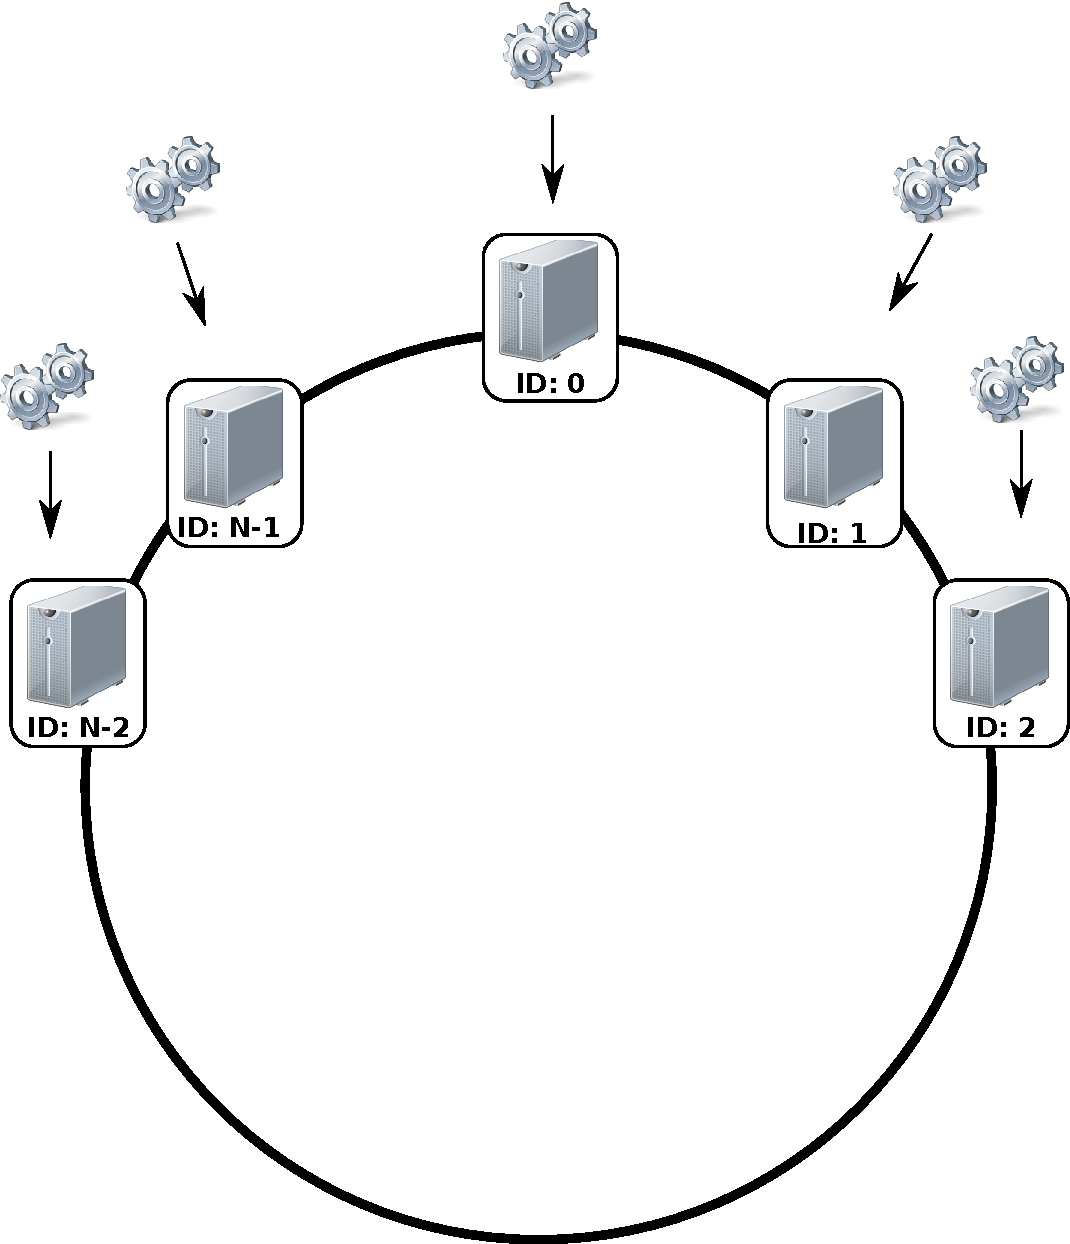
\includegraphics[width=0.8\textwidth,clip=true,trim=0px 225px 0px 0px]{resources/drawing.pdf}
\caption{A ring structured network}
\label{figring}
\end{figure}

The performance of a forwarding algorithms is measured by the average number of nodes a job must visit before being executed. The goal of the algorithms is to minimize this number by spreading the load evenly along the ring. 

\subsection{Forwarding algorithms}
Nodes that must forward a job will choose another node of the ring. Nodes have no information about other nodes, so it has no idea whitch nodes are idle or busy. The algorithms are grouped into two categories: forward to neighbour and forward anywhere.
The first techniques allows a busy node to forward an incoming job to either its left or its right neighbor, where the latter may forward these jobs to any node in the ring. 
Since the amount of dropped jobs is equal for each forwarding algorithm. These jobs will be ignored when computing the average number of forwards. One should note that the loss rate of jobs in the system is the same as the Erlang-b loss rate.

\subsection{Forward to neighbour}
\subsubsection*{Forward right}
A busy node using this technique will forward a job to its right neighbour. The job will keep travelling in this direction until an idle node is found, where it will be processed or it has visited all nodes, when it will be dropped. Unless otherwise noted, this algorithms is used as baseline in all further tests. This algorithm does not use any space in the job's metadata, nor must nodes save states.

\subsubsection*{Left/Right forward}
A variant to the previous algorithm is the Left/Right forward technique. Instead of forwarding each job to its right neighbour, a busy node will alternate the direction after forwarding such a job. To avoid a job coming back, this initial direction is saved in the job's metadata. Busy nodes receiving a job from another neighbour must forward it the same direction as specified in the job's metadata. This algorithms requires the 1 bit representing the direction in the job's metadata, it also needs the save 1 bit state information in each nodes to keep track of the last direction a new job was forwarded to.

\subsubsection*{Random Left/Right forward with parameter $p$}
This technique is a variant of the Left/Right forward algorithm. However, instead of alternating the direction for each new job, a node will forward a job to its right with probability $p$ and to its left with probability $1-p$. As the previous technique, the direction is saved in the job's metadata and subsequent nodes must maintain this direction when forwarding. On the contrary, nodes do not need to save state information.

\subsubsection*{Position-dependant forwarding}
As shown in figure \ref{figring}, each node in the ring has an unique ID. Except the for node with id $0$ and $N-1$, neigbouring are succeeding. When nodes uses this algorithm, nodes will always forward a new job in the same direction: to the right when the node's id is even, to the left otherwise. As previous algorithms, the direction is saved in the job's metadata and this direction must be used if other nodes must forward the job. The initial direction of incoming jobs can be derived from the node's ID, therefore the node needs no state information.

\subsection{Forward anywhere}
The ring strucure can be used in real networks, however in many cases the ring is no more than a virtual overlay over another structure (e.g. the internet). In these networks each node is able to connect each other node directly and more sophisticated forwarding algorithms can be used.

\subsubsection*{Random unvisited}
The Random unvisited algorithm is the most basic algorithm in this category. Everytime a job must be forwarded, a list of unvisited nodes is generated and a random node is choosen from that list. The current node is added to the list of visited nodes, which is found in the job's metadata. This list can be saved using $N$ bits.

\subsubsection*{Coprime offset}
Another algorithm is Coprime offset. This algorithm generates a list of all numbers smaller than $N$, and coprime to $N$. The first time a job is forwarded the next number of this list is selected. This is the job's forward offset and saved in the its metadata. When a job is forwarded, it is sent exactly this many hops farther. Because this number and $N$ are coprime, it will visit all nodes exactly once before being returned to its originating node. 

Example:
Consider a ring size of $N=10$ in which every node is busy. The list of coprimes is than generated: ${1, 3, 7, 9}$. Assume a job arrives at node $3$ and the last time node $3$ forwarded a job it was given offet $1$.
Because this node is busy, the next number on the list ($3$) is selected and saved in the job's metadata. All nodes are busy so the job visits these nodes before being dropped: $3$ (arrival), $6, 9, 2, 5, 8, 1, 4, 7, 0$. Node $0$ will drop the job because the next node would be $3$, which is the node on wich the job arrived.

Because the list of coprimes can be regenerated each time a job arrives, it must not be saved. Both the job and the node must keep an index to a coprime. The size of this list $\tau(N)$ thus an index to an element in this list requires $\lceil log_2 \tau(N) \rceil$ bits.

\subsubsection*{Random Coprime offset}
The Random Coprime offset algorithm is almost equal to Coprime offset. The difference between them is the decision of the offset value. Where it is the next number on the list in Coprime offset, a random value is taken from the list when using Random Coprime offset. As Coprime offset, the offset must be saved in the job's metadata. Since the offset for incoming jobs is choosen at random, the nodes do not need to keep state information.

\subsection{Properties of Algorithms}

We have reviewed some of the basic properties for each algorithm, they can be found in table \ref{tabprops}. The function $\tau(N)$ represents the number of values smaller than $N$ and coprime to $N$.

\[ \tau(N) = \sum_{0 < p < N, p \perp N} 1\]
Note that this value is upper bound by $N-1$ and equals $N-1$ when $N$ is prime.

\footnotetext[1]{For Random Left/Right forward for which $p \neq 0.5$, the probabilty of each path is different.}
\begin{table}[h!]
\hspace{-0.12\textwidth}
\begin{tabular}{|p{0.30\textwidth}|p{0.10\textwidth}|p{0.18\textwidth}|p{0.18\textwidth}|p{0.18\textwidth}|p{0.18\textwidth}|} \cline{2-6}
\multicolumn{1}{l|}{}		& Size known	& First forward	& Possible paths	& Space requirement (job)	& Space requirement (node) \\ \hline
Forward Right				& N				& 1				& 1					& 0							& 0		\\ \hline
Left/Right forward			& N				& 2				& 2					& 1							& 1		\\ \hline
Random Left/Right forward (p) & N			& 2				& 2 $^($\footnotemark$^)$ & 1					& 0		\\ \hline
Position dependant forward	& N				& 1				& 1					& 1							& 0		\\ \hline
Random unvisited			& Y				& $N-1$			& $(N-1)!$			& $N$	& 0		\\ \hline
Coprime offset				& Y				& $\tau(N)$		& $\tau(N)$ 		& $\lceil log_2 \tau(N) \rceil$	& $\lceil log_2 \tau(N) \rceil$ \\ \hline
Random Coprime offset		& Y				& $\tau(N)$		& $\tau(N)$			& $\lceil log_2 \tau(N) \rceil$	& 0		\\ \hline
\end{tabular}
\caption{Properties of forwarding algorithms}
\label{tabprops}
\end{table}

\begin{description}
\item[Size known] Represents whether the size of the ring must be known to the nodes in order to function.
\item[First forward] When the node on which the incoming job arrives is busy, this number represents the number of candidates to which the node can forward the job.
\item[Possible paths] Assuming the system is saturated, this number represents the number of possible paths a job can travel until being dropped. The probabilty of each path is the same (unless otherwise noted).
\item[Space requirement (job)] This value represents the number of bits required in the job's metadata.
\item[Space requirement (node)] This value represents the number of bits required to save the node's state information.
\end{description}

\section{Simulation}
\label{secsimulation}
To evaluate the different algorithms discussed in the previous section, 2 methods will be used. Firstly using a simulation, the second method is the numerical evaluation of this simulation using MATLAB. The validation method is further discussed in section \ref{secvalidation}.

The simulation is accomplished using a custom simulator. A continuous time simulator is written in C++, using no external requirements but the STL and OpenMP \cite{OPENMP}. The source code of the simulator can be found in appenix \ref{sourcecode} or at \url{http://code.google.com/p/powerofpaths/}.

The simulator can be controlled using a command line interface of which the usage is described below:
\lstset{language=sh,caption={Simulator usage description}}
\begin{lstlisting}
Usage: -r -s long -j double -a double -n long -p long -l long -t long -h type
	-r	Random seed
	-s	Set seed			(default: 0)
	-j	Job length			(default: 1.0)
	-a	Load				(default: 1.0)
	-n	Ring size			(default: 100)
	-c	Processing units per node	(default: 1)
	-p	Print progress interval		(default: -1 - disabled)
	-l	Simulation length		(default: 3600)
	-t	Repetition			(default: 1)
	-h	Print this help
	 type	right | switch | randswitch | evenswitch | prime | randprime | randunvisited | totop
\end{lstlisting}

\subsection{Measure}
The goal of the algorithms is to distribute the jobs evenly along the ring. This implies that the number of nodes a job must visit should be low. As a measure for our experiments, we will be using the average number of times a job is forwarded before it is executed. Since the number of forwards of a job that could not be executed is the same for each algorithm (i.e. $N-1$: traversing each link but one), and the loss rate of each algorithm is the same (because forwards are instantaneous), we will not take these jobs into account when computing the average.

It is clear that when the system load approaches $0$, the probability that a node is busy will also approach $0$ and the average number of forwards will therefore also approach $0$. On the other hand, when the load approaches $\infty$, each node's probability of being busy will approach $1$ and therefore the number of forwards will be $N-1$ and the job will fail. A system with load $> 1$ is called an overloaded system. For the purpose of this thesis, only loads up to $1$ are discussed.

We will compare each algorithm to a baseline result. The baseline used in this thesis is the Forward right algorithm. This means that each graph will show its result relative to the Forward right results. The results given by the simulator were obtained using a ring size of 100 and using a random seed for each run.

The absolute performance of the baseline algorithm is shown in figure \ref{baseline}.

\begin{figure}[h!tb]
\centering
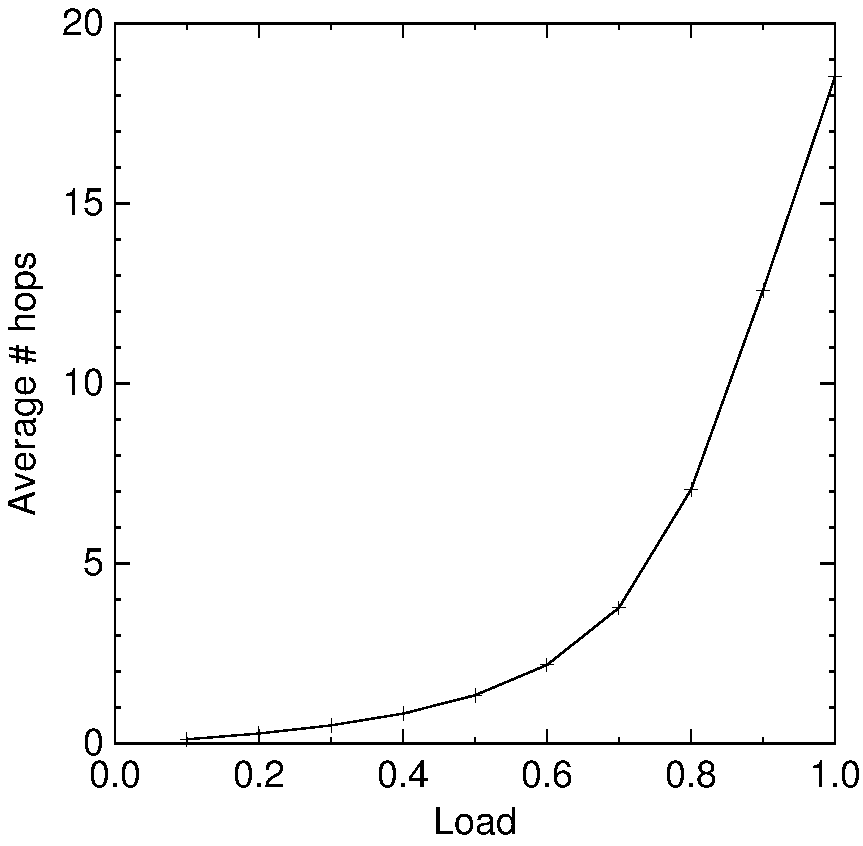
\includegraphics[width=0.6\textwidth]{data/right.pdf}
\caption{The Forward Right baseline result}
\label{baseline}
\end{figure}

\subsection{Results}
\label{simresults}

\subsubsection*{Left/Right Forward}
It is intuitively clear that alternating the forwarding direction of incoming jobs should distribute the load better than keeping the same direction, certainly under temporary local heavy load. Figure \ref{figlr} shows the improvement made by the Left/Right forward algorithm over the Forward right method. The performance gain is at least 1\% and up to over 4\% under medium load.

\begin{figure}[h!tb]
\centering
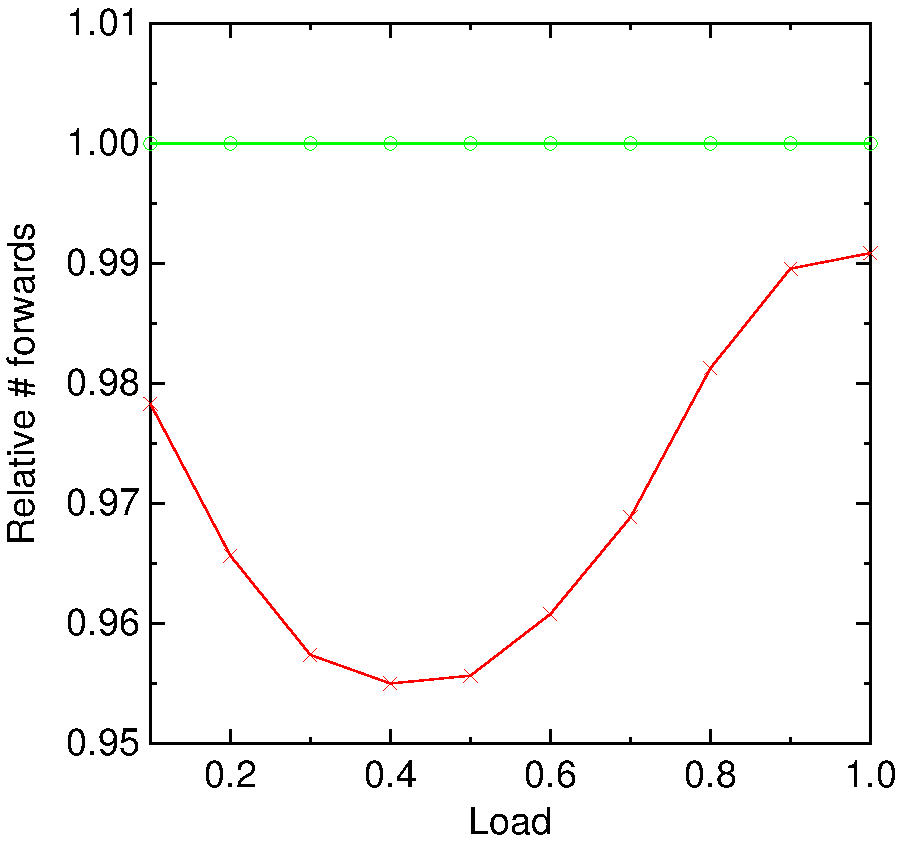
\includegraphics[width=0.6\textwidth]{data/switchright.pdf}
\caption{Left/Right}
\label{figlr}
\end{figure}


\subsubsection*{Random Left/Right forward with parameter $p$}
For $p=0.5$, one would expect the results of this algorithm being similar to those obtained in the previous simulation. However, it seems the small change in the algorithm worsened the results significantly.

\begin{figure}[h!tb]
\centering
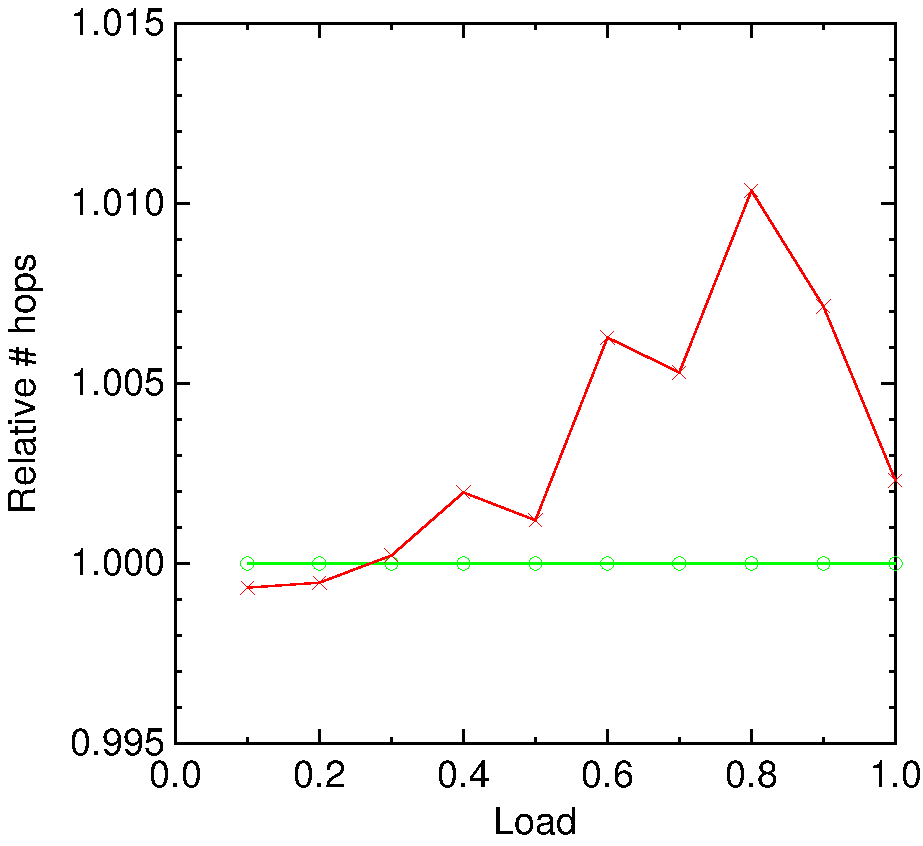
\includegraphics[width=0.6\textwidth]{data/randswitchright.pdf}
\caption{Random Left/Right forward with parameter $0.5$}
\label{figrandswitch}
\end{figure}

Figure \ref{figrandswitch} shows the results of this algorithm for $p=0.5$. For $p=0$, the algorithm is equal to the Forward Right algorithm. Hence, we should investigate how different values of $p$ influence the final results. Figure \ref{figrandswitchp} shows the results obtained for $0 \leq p \leq 0.5$. We see there is no value of $p$ for which this algorithms performs better than Forward Right.

\begin{figure}[h!tb]
\centering
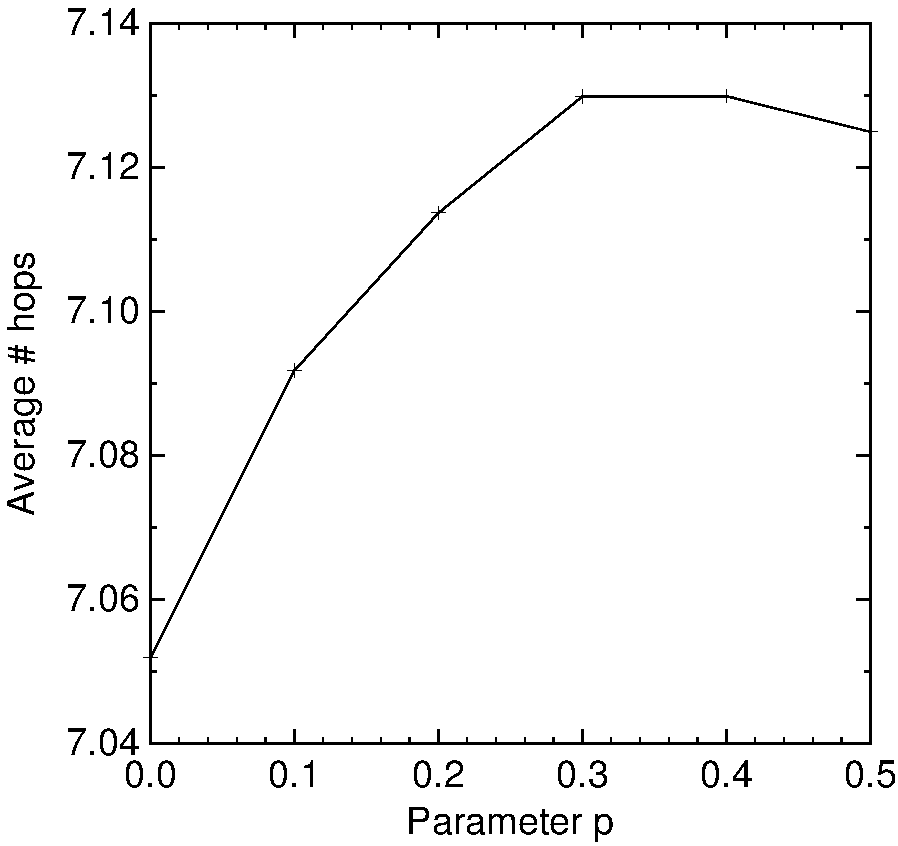
\includegraphics[width=0.6\textwidth]{data/randswitchp.pdf}
\caption{Random Left/Right forward with load $0.8$}
\label{figrandswitchp}
\end{figure}

\subsubsection*{Position-dependant forwarding}
This technique groups every 2 nodes into small virtual clusters. When a job arrives at a busy node, the job will be forwarded to the other node in this cluster. Jobs leaving a cluster will seem to do this in a random direction ($p=0.5$). Since the load is concentrated per cluster instead of being distributed over the whole system, this technique performs worse than other techniques The results are represented in figure \ref{figevenswitch}.

\begin{figure}[h!tb]
\centering
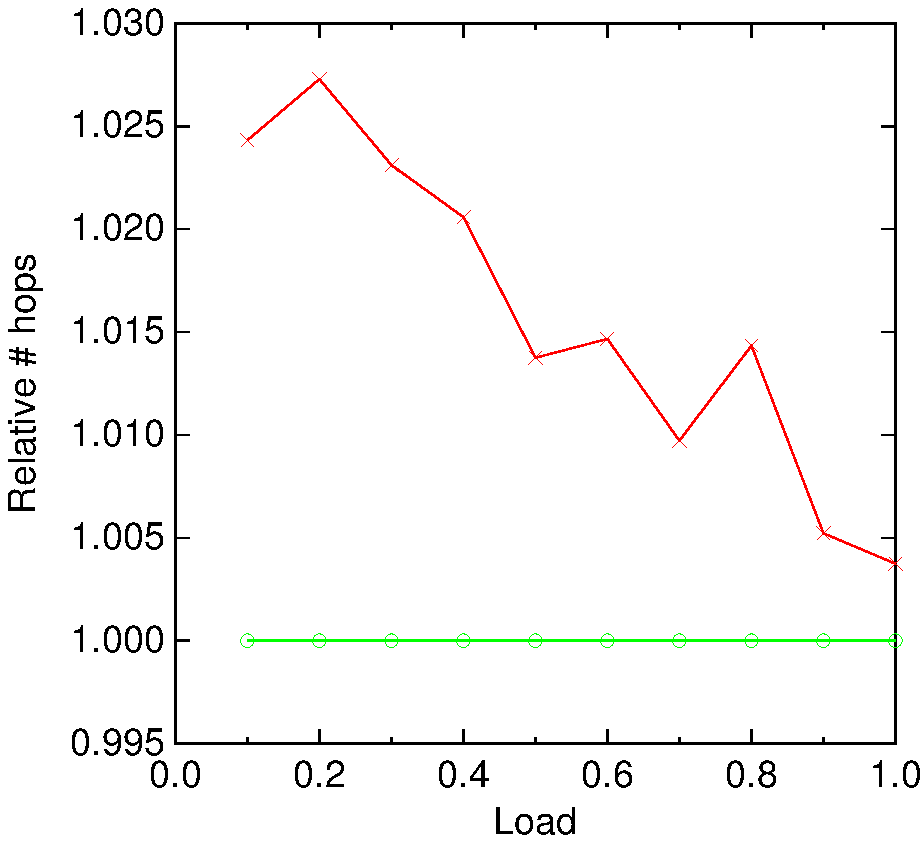
\includegraphics[width=0.6\textwidth]{data/evenswitchright.pdf}
\caption{Position-dependant forwarding}
\label{figevenswitch}
\end{figure}


\subsubsection*{Random unvisited}
This algorithm is not bound to its neighbors when forwarding a job. Lifting this constraint allows a serious performance boost. ***********

This algorithm in the most straight forward and is the best performing from any of these techniques. However, it should be noted that each visited node must be stored into the job's metadata, at least $N$ bits should be available to store this information.

\begin{figure}[h!tb]
\centering
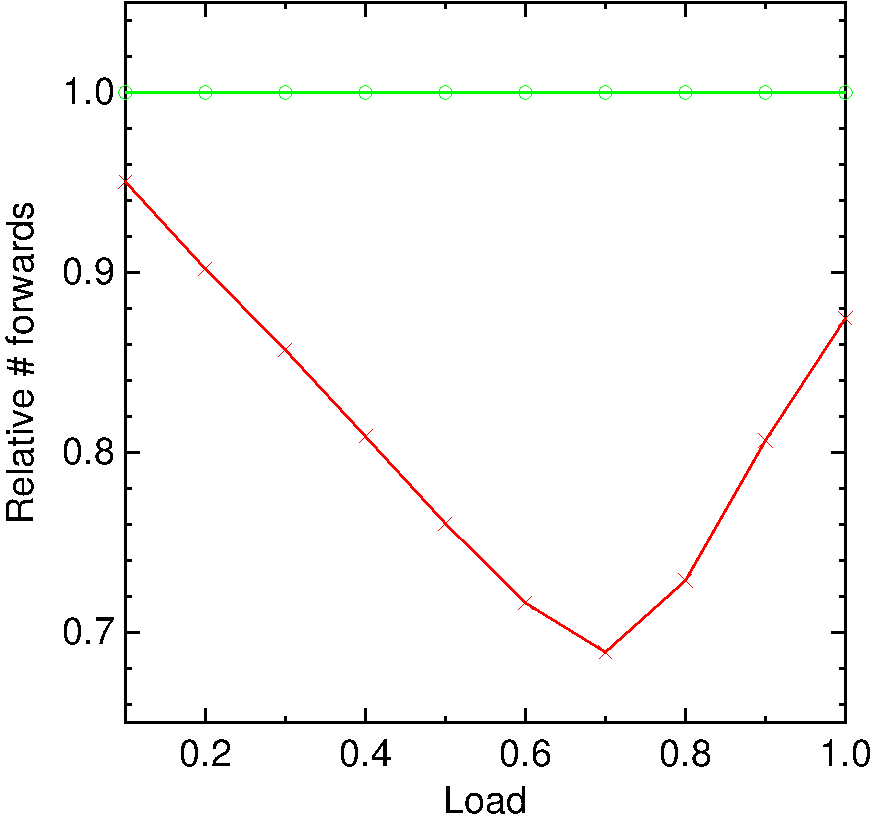
\includegraphics[width=0.6\textwidth]{data/randunvisitedright.pdf}
\caption{Random unvisited forwarding}
\label{figrandunvisited}
\end{figure}

Figure \ref{figrandunvisited} shows the results of this algorithms. It is the first algorithm tested that could forward jobs to nodes other than its neighbors. We see that lifting that constraint allows a serious performance boost.

\subsubsection*{(Random) Coprime offset}
Two other algorithms that are not restricuted to forwarding to a neighbor are Coprime offset and Random Coprime offset. Figure \ref{figprimes} shows the results of both these algorithms. The difference of these algorithms with themselves and the random unvisited algorithms is not clearly visible when comparing both to the Forward Right algorithm. To put these results in perspective, we included figure \ref{figruprp} where Coprime offset and Random Coprime offset are depicted relative to Random unvisited. Although the difference is small, it seems the Random unvisited algorithm shows a better performance than the other two. However, Coprime offset and Random Coprime offset require $\lceil log_2 N \rceil$ bits in the job's metadata instead of $N$ for Random unvisited.

\begin{figure}[h!tb]
        \begin{subfigure}[b]{0.5\textwidth}
                \centering
                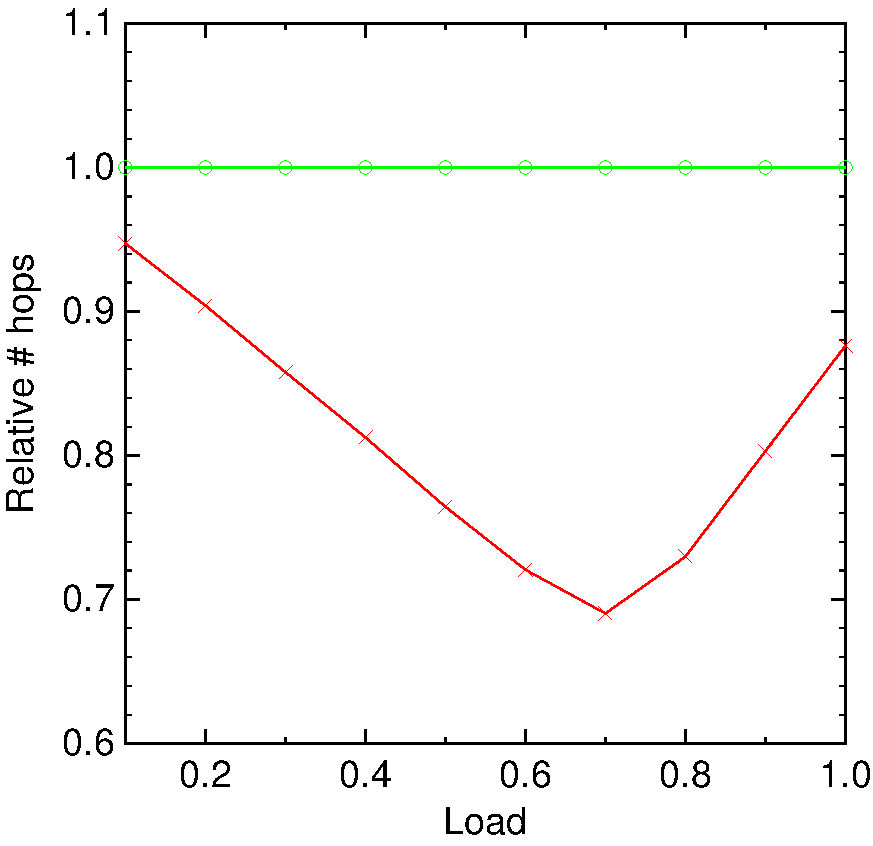
\includegraphics[width=\textwidth]{data/primeright.pdf}
                \caption{Coprime offset}
        \end{subfigure}
        \begin{subfigure}[b]{0.5\textwidth}
                \centering
                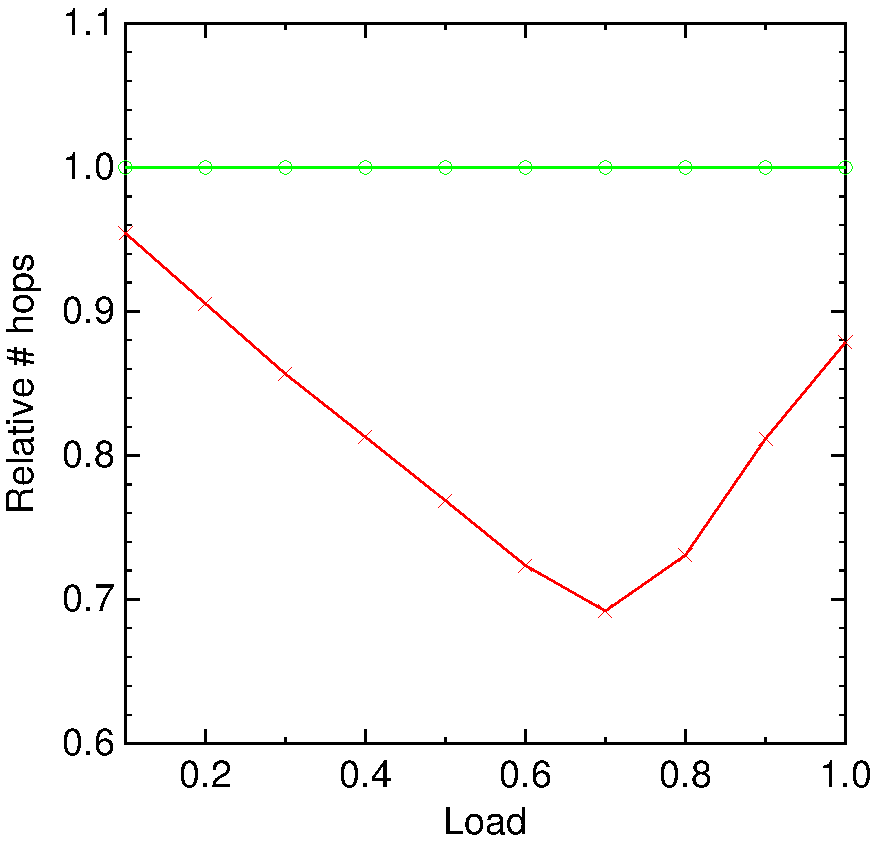
\includegraphics[width=\textwidth]{data/randprimeright.pdf}
                \caption{Random Coprime offset}
        \end{subfigure}
\caption{(Random) Coprime offset}
\label{figprimes}
\end{figure}

\begin{figure}[h!tb]
\centering
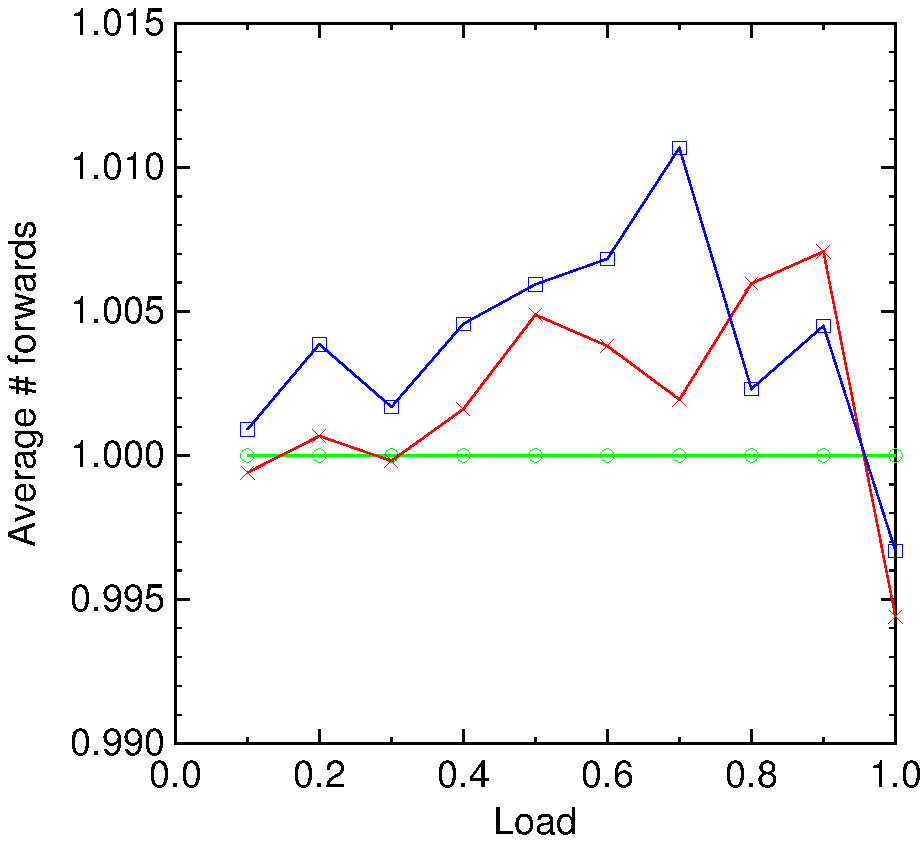
\includegraphics[width=0.8\textwidth]{data/randunvisited_prime_randprime.pdf}
\caption{Random unvisited (green), Coprime offset (blue), Random Coprime offset (Red)}
\label{figrandunvisited}
\end{figure}

\subsection{Multiple execution units}
So far, all simulations were executed using 1 cpu per server. This is not a realistic assumption for most distributed systems. This section is intended to research the behaviour of the algorithms when using multiple cpu's, and comparing the results to a system with 1 cpu per server, and to each other.

Per algorithm, the two simulations are performed and compared, see table \ref{tabcpus} for more information about the tests.
\begin{table}[h!]
\centering
\begin{tabular}{|p{0.2\textwidth}|p{0.4\textwidth}|p{0.4\textwidth}|} \hline
Algorithms & \multicolumn{2}{|p{0.8\textwidth}|}{Forward right, Left/Right, Random left/right (0.5), Random unvisited, Random Coprime offset} \\ \hline
Ring size & 100 & 25 \\ \hline
Cpu's per node	& 1 & 4 \\ \hline
Load	& \multicolumn{2}{|c|}{$0.1 - 1.0$} \\ \hline
\end{tabular}
\caption{Comparison of algorithms using multiple cpu's per server}
\label{tabcpus}
\end{table}

Since the ring size for the second test is 25 instead of 100, the number of forwards of the second test will be multiplied by 4 to get meaningful results. This actually makes sense because a job that is forwarded once has encountered 4 busy cpu's. The baseline for the tests is the basic result of the algorithm found in section \ref{simresults}, where the second test is drawn relative to the basic result.

\begin{figure}
        \begin{subfigure}[b]{0.5\textwidth}
                \centering
                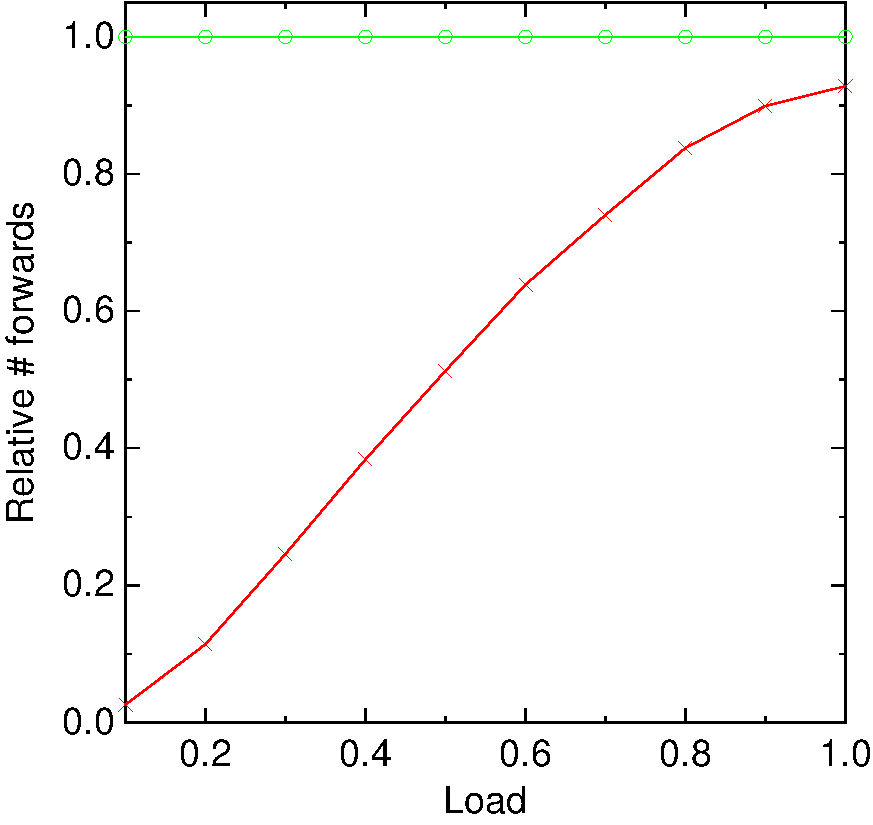
\includegraphics[width=\textwidth]{data/4rightright.pdf}
                \caption{Forward right}
        \end{subfigure}
        \begin{subfigure}[b]{0.5\textwidth}
                \centering
                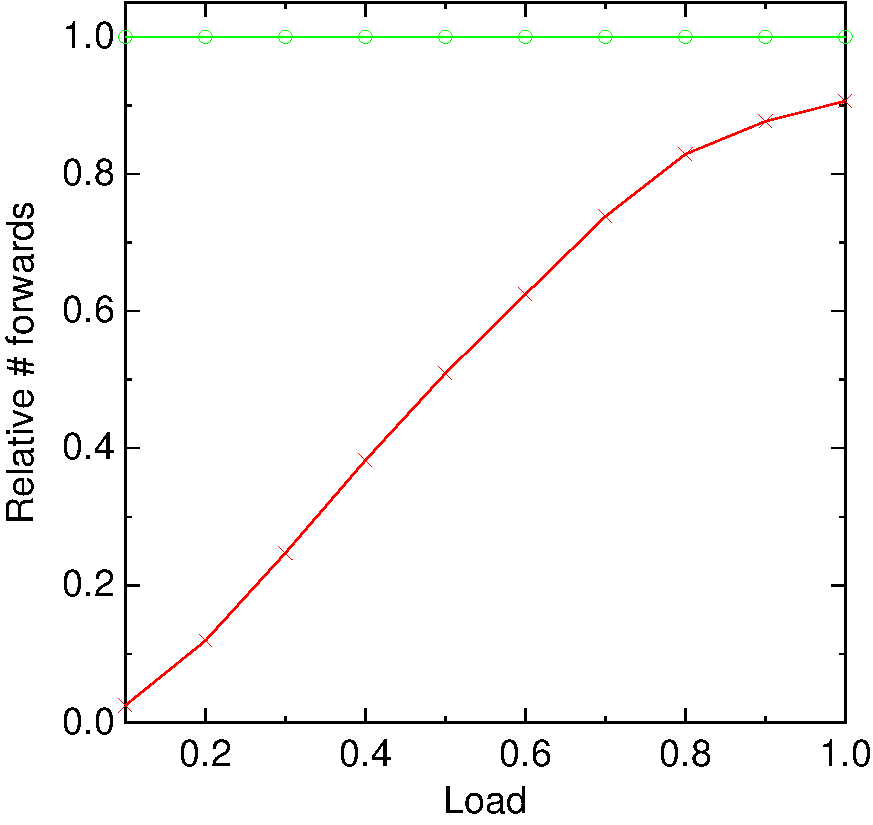
\includegraphics[width=\textwidth]{data/4switchswitch.pdf}
                \caption{Forward Left/Right}
        \end{subfigure}
        
        \begin{subfigure}[b]{0.5\textwidth}
                \centering
                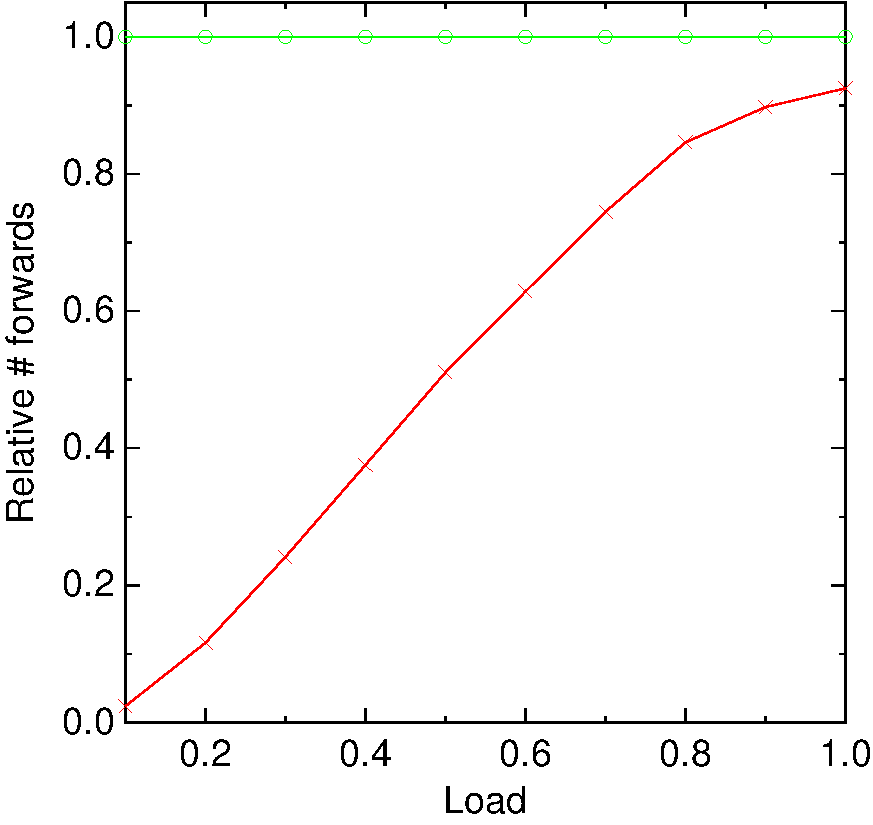
\includegraphics[width=\textwidth]{data/4randswitchrandswitch.pdf}
                \caption{Random Left/Right (0.5)}
        \end{subfigure}
        \begin{subfigure}[b]{0.5\textwidth}
                \centering
                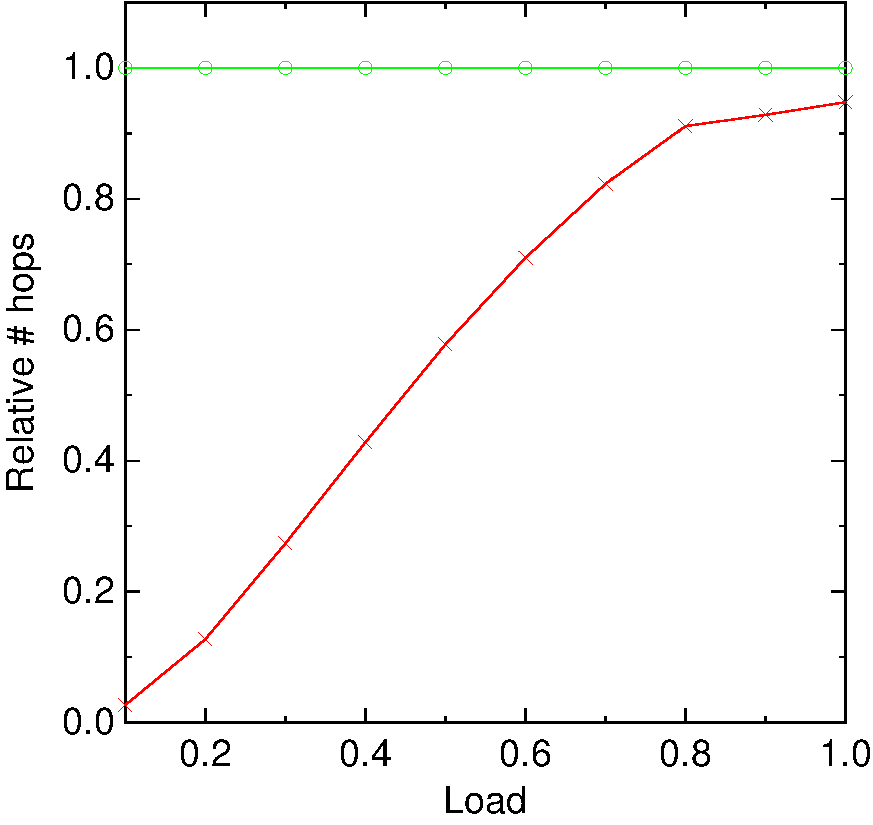
\includegraphics[width=\textwidth]{data/4randunvisitedrandunvisited.pdf}
                \caption{Random unvisited}
        \end{subfigure}
        
        \begin{subfigure}[b]{0.5\textwidth}
                \centering
                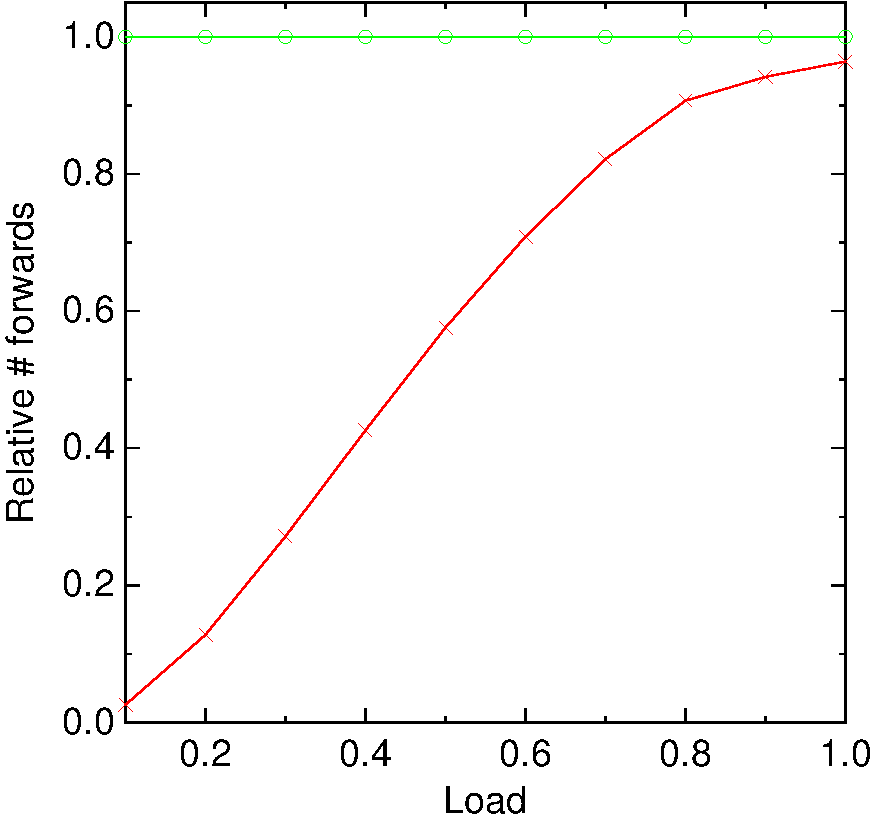
\includegraphics[width=\textwidth]{data/4randprimerandprime.pdf}
                \caption{Random Coprime offset}
        \end{subfigure}
        \caption{4 cpu's per server versus 1}\label{figcpus}
\end{figure}

Figure \ref{figcpus} shows the performance of 4 cpu's versus 1 cpu for different algorithms. For each of the tested algorithms, we see the same result. This means the results of each algorithm is influenced in the same way when using multiple cpu's per server. We can use this knowledge to generalize the results of section \ref{simresults}.

Since we assume each algorithm is infuenced the same way, let us investigate one of them in depth. We will try to transform the results of an algorithm with ring size $N$ and $1$ cpu per server into the results of the same algorithm with ring size $N/c$ and $c$ cpu's per server. The load of the system should be the same.

Let $d$ be the distribution of the number of forwards, stored as a rowvector. We will build a transformation vector $M$ in the form $[ \lfloor 0/c \rfloor,  \lfloor 1/c \rfloor, \ldots, \lfloor (N-1)/c \rfloor]'$. This vector represents the number of times a job would be forwarded if there would be $c$ cpu's per server. $d*M$ equals the average number of forwards when using such a system. To negate the dropped jobs, the results must be weighted for only the completed jobs.
In our example, we will transform the results of the Forward Right algorithm using ring size $N=10$ and 1 cpu into the results of a ring with size $N=5$ and $c=2$ cpu's per server, see table \ref{tabcpus} for a worked out example and figure \ref{figcpusmatch} for a comparison of the transformation and a real simulation.


\begin{table}
\centering
\begin{tabular}{|r|l|r|l|} \hline
\# hops & Distribution & M & Result \\ \hline
0 & 0.5092 & 0 & 0 \\ \hline
1 & 0.2118 & 0 & 0 \\ \hline
2 & 0.1082 & 1 & 0.1082 \\ \hline
3 & 0.0609 & 1 & 0.0609 \\ \hline
4 & 0.0363 & 2 & 0.0726 \\ \hline
5 & 0.0224 & 2 & 0.0449 \\ \hline
6 & 0.0142 & 3 & 0.0426 \\ \hline
7 & 0.0091 & 3 & 0.0272 \\ \hline
8 & 0.0058 & 4 & 0.0233 \\ \hline
9 & 0.0037 & 4 & 0.0147 \\ \hline
Total &  0.9816 & &  0.3944 \\ \hline
Weighted total & \multicolumn{3}{|c|}{$0.3944/0.9816 = 0.4018 $} \\ \hline
Simulation result & \multicolumn{3}{|c|}{$0.4171$} \\ \hline
\end{tabular}
\caption{Comparison when load=0.5}
\label{tabcpus}
\end{table}

\begin{figure}[h!tb]
\centering
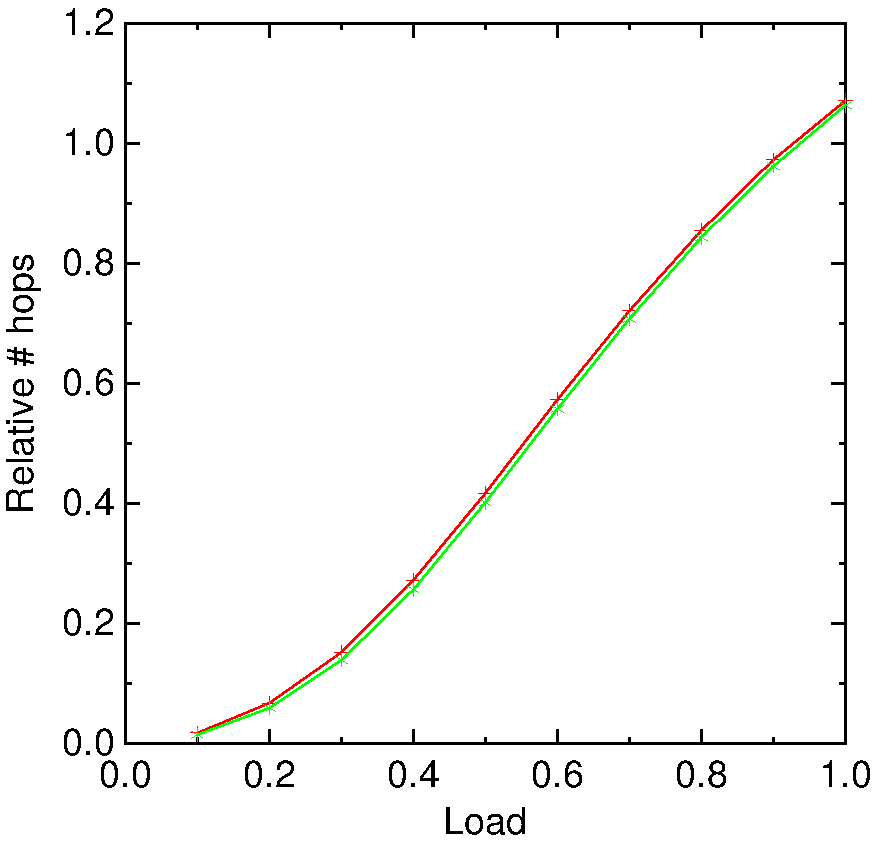
\includegraphics[width=0.8\textwidth]{data/right_5_2.pdf}
\caption{Multiple cpu's result derived of the result for 1 cpu (green) versus the actual simulation result (red)}
\label{figcpusmatch}
\end{figure}


\section{Numerical Validation}
** BEPAALDE ALGORITMES NIET BESPROKEN, WAAROM?

\label{secvalidation}

To validate the results obtained in the previous section, we modelled the scheduling-techniques into Markov Chains. Using the steady state distribution of these chains, we can derive the average number of hops and the average loss.
For $N$ nodes in a ring, the markov chain consists of $2^N$ states, where the $n$-th bit represents whether the $n$-th server is busy ($1$) or idle ($0$). To optimize the computation time and memory requirements, we used sparse matrixes for the validation. The validation code is written in MATLAB, it can be found in appendix \ref{matlabcode} or on \url{http://code.google.com/p/powerofpaths/}.

The validation of the results happens in a different environment than the simulation. Because of the non-polynomial execution time of the algorithm, the size of the ring is reduced to $10$. Therefore, the results of this validation are smaller but the relative results are still relevant.

\subsection{Forward Right}
\label{validateright}
Modelling a technique into a Markov Chain is an easy operation for most algorithms. The example given below is for a ring of 3 nodes. For convenience, the states are represented by their binary form.

\[ Q =
  \begin{blockarray}{ccccccccc}
    & 000 & 001 & 010 & 011 & 100 & 101 & 110 & 111 \\
    \begin{block}{c[cccccccc]}
    000 & -3 \lambda & \lambda & \lambda & 0 & \lambda & 0 & 0 & 0 \\
    001 & \mu & -3\lambda-\mu & 0 & \lambda & 0 & 2\lambda & 0 & 0 \\
    010 & \mu & 0 & -3\lambda-\mu & 2\lambda & 0 & 0 & \lambda & 0 \\
    011 & 0 & \mu & \mu & -3\lambda-2\mu & 0 & 0 & 0 & 3\lambda \\
    100 & \mu & 0 & 0 & 0 & -3\lambda-\mu & \lambda & 2\lambda & 0 \\
    101 & 0 & \mu & 0 & 0 & \mu & -3\lambda-2\mu & 0 & 3\lambda \\
    110 & 0 & 0 & \mu & 0 & \mu & 0 & -3\lambda-2\mu & 3\lambda \\
    111 & 0 & 0 & 0 & \mu & 0 & \mu & \mu & -3\mu \\
    \end{block}
  \end{blockarray}
\]

\begin{figure}[h!tb]
\centering
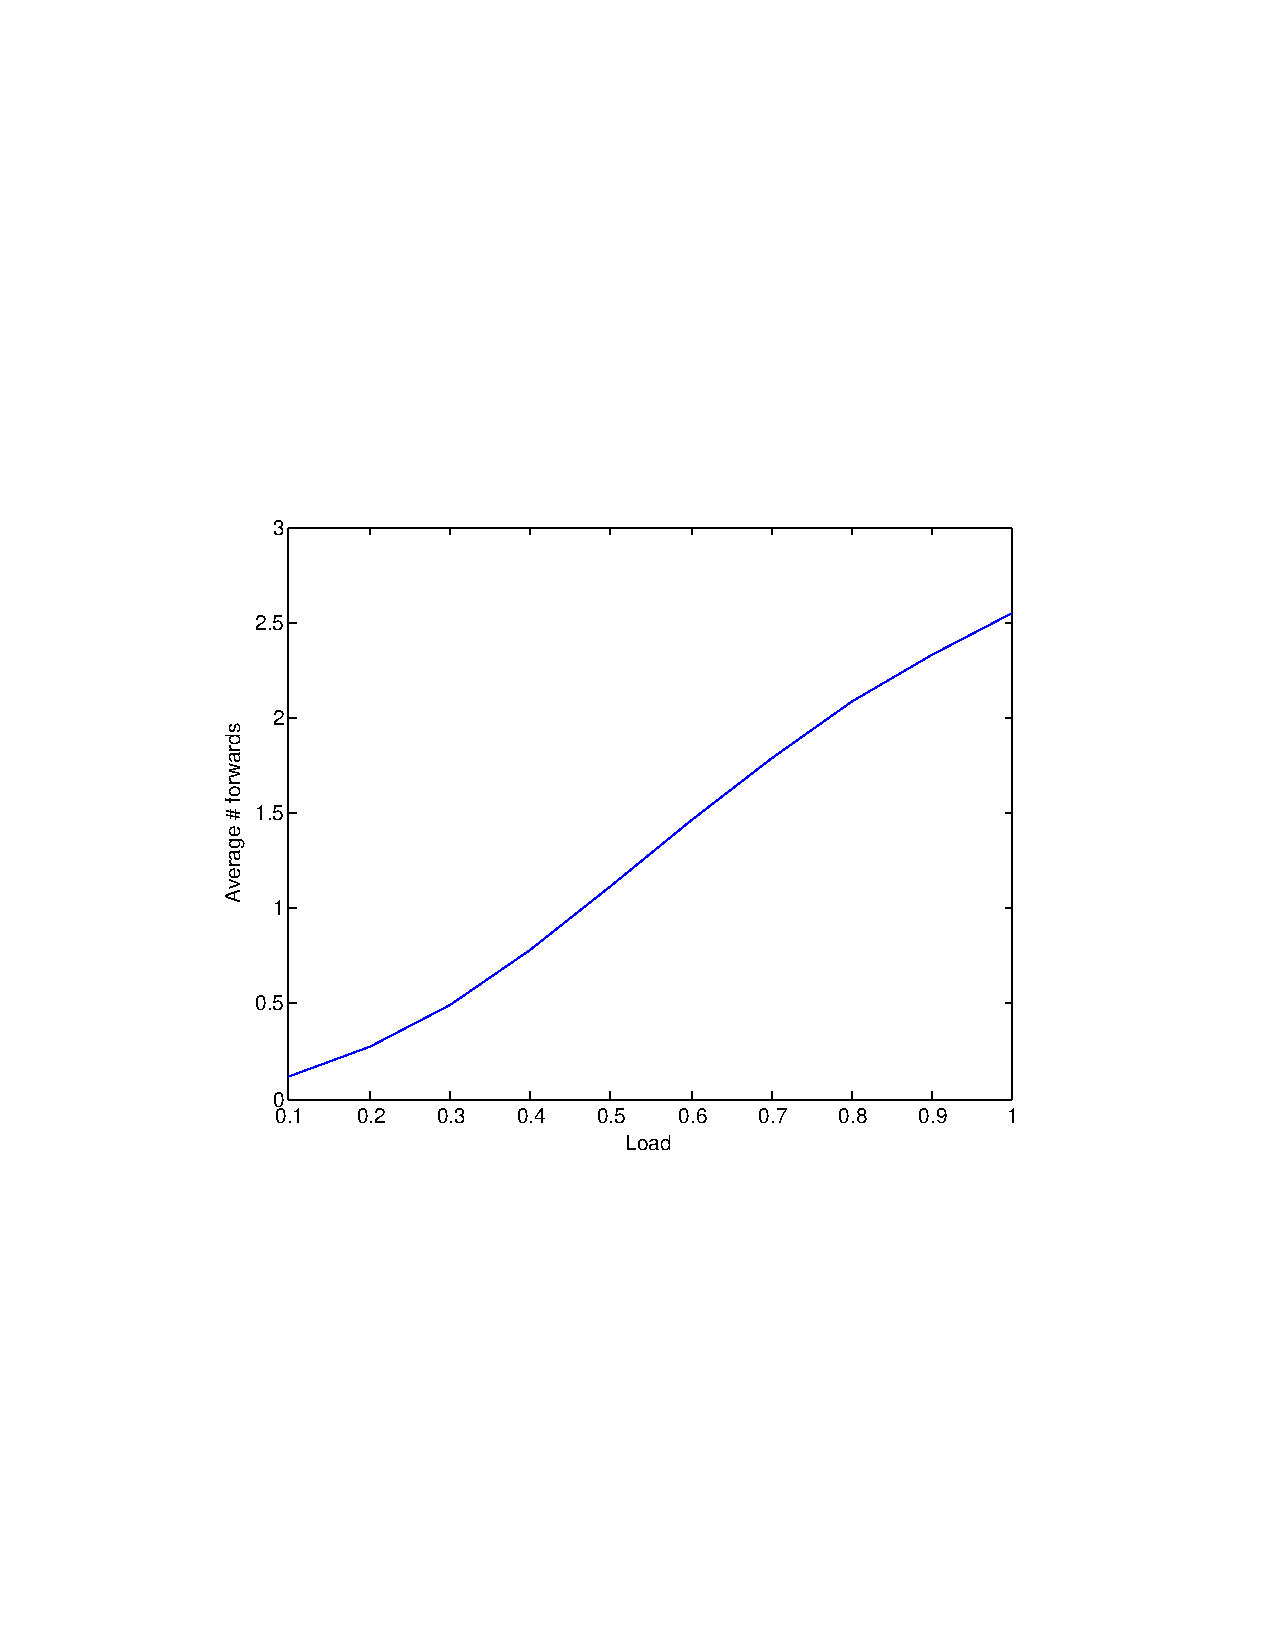
\includegraphics[clip=true, trim=9em 24em 9em 24em, width=0.9\textwidth]{resources/plotright.pdf}
\caption{Validation of Forward right}
\label{validright}
\end{figure}

Analogue to the simulation section, this method will be the baseline result in our other results.

\subsection{Random Left/Right forward with parameter $p$}
This matrix is very similar to the one above. But we need to take into account the parameters $p$ and $1-p$ instead of $1$ and $0$.

\[ Q =
  \begin{blockarray}{ccccccccc}
    & 000 & 001 & 010 & 011 & 100 & 101 & 110 & 111 \\
    \begin{block}{c[cccccccc]}
    000 & -3 \lambda & \lambda & \lambda & 0 & \lambda & 0 & 0 & 0 \\
    001 & \mu & -3\lambda-\mu & 0 & (2-p)\lambda & 0 & (1+p)\lambda & 0 & 0 \\
    010 & \mu & 0 & -3\lambda-\mu & (1+p)\lambda & 0 & 0 & (2-p)\lambda & 0 \\
    011 & 0 & \mu & \mu & -3\lambda-2\mu & 0 & 0 & 0 & 3\lambda \\
    100 & \mu & 0 & 0 & 0 & -3\lambda-\mu & (2-p)\lambda & (1+p)\lambda & 0 \\
    101 & 0 & \mu & 0 & 0 & \mu & -3\lambda-2\mu & 0 & 3\lambda \\
    110 & 0 & 0 & \mu & 0 & \mu & 0 & -3\lambda-2\mu & 3\lambda \\
    111 & 0 & 0 & 0 & \mu & 0 & \mu & \mu & -3\mu \\
    \end{block}
  \end{blockarray}
\]

The lumped matrix (section \ref{lump}) of $Q$ is equal to the lumped matrix of the example above, i.e. the matrix defines the exact same behaviour. However, for $N > 6$ the matrices and so the results of the steady state distribution begin to differ.

\begin{figure}[h!tb]
\centering
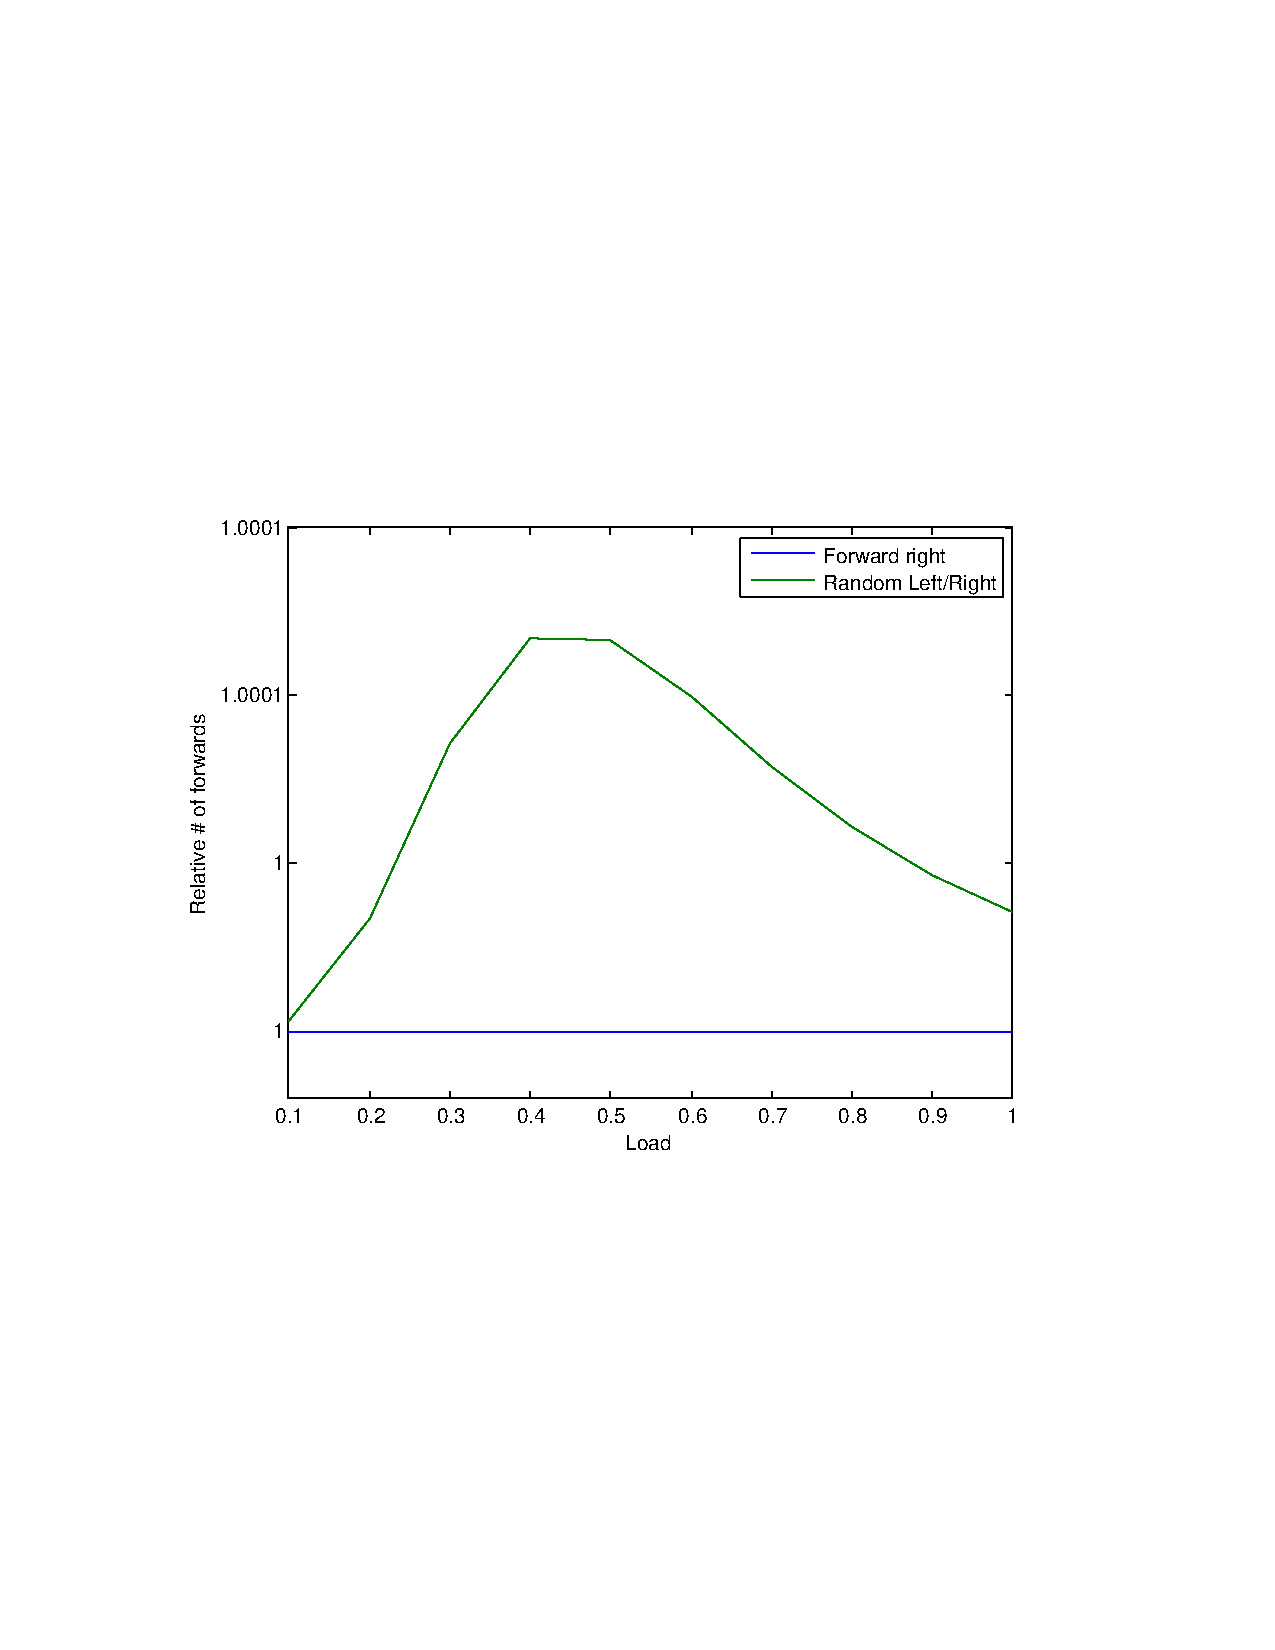
\includegraphics[clip=true, trim=9em 24em 9em 24em, width=0.9\textwidth]{resources/plotrandlr.pdf}
\caption{Validation of Random Left/Right with p=$0.5$}
\label{validrlr}
\end{figure}

As in the simulation section, we have validated the results for different values for $p$. These results are shown in figure \ref{validrlrp}.

\begin{figure}[h!tb]
\centering
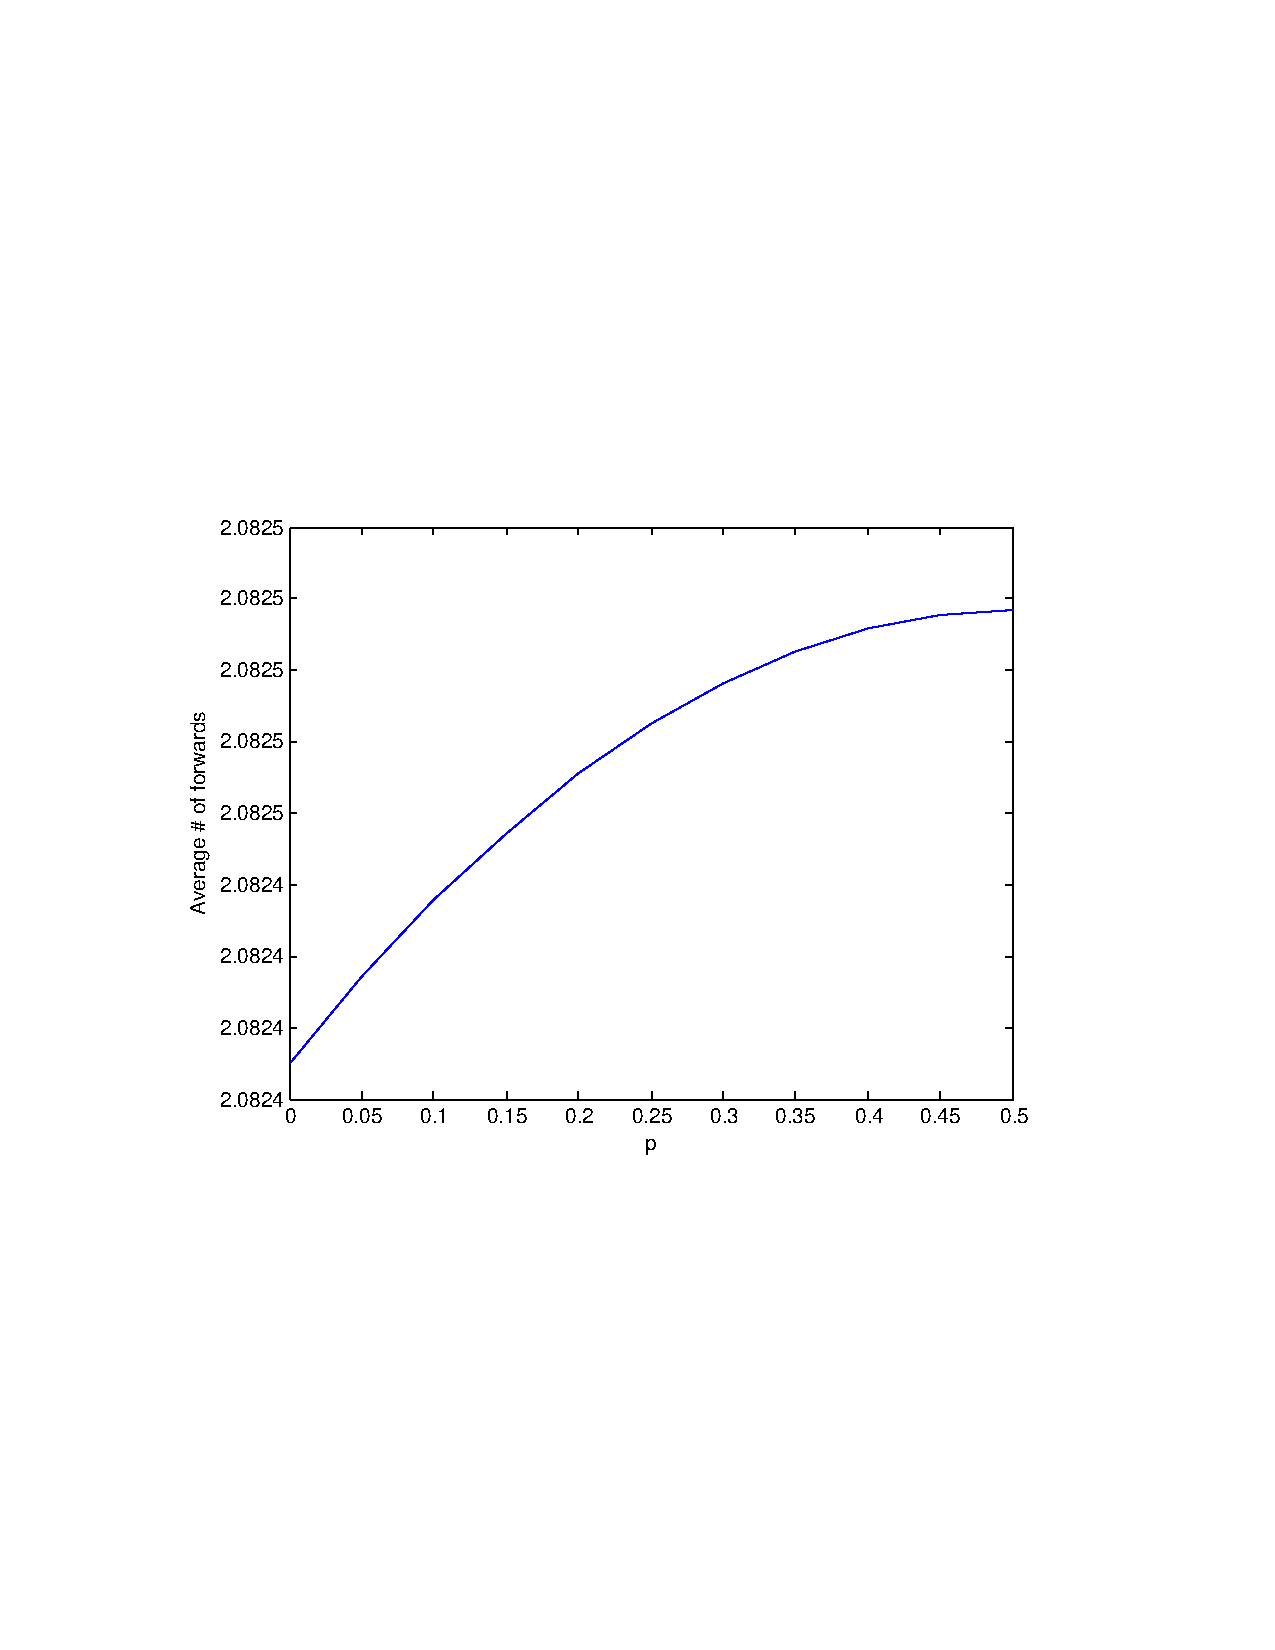
\includegraphics[clip=true, trim=9em 24em 9em 24em, width=0.9\textwidth]{resources/plotrandlrp.pdf}
\caption{Performance of Random Left/Right with load$=0.8$}
\label{validrlrp}
\end{figure}

\subsection{Random Coprime offset}
Modelling this technique yields different results for various ring sizes. The performance of this algorithm is very dependant on the number of coprimes that can be used. This technique yields the same results as Forward Right for ring sizes of up 4. For $N = 3$, the matrix $Q$ is identical to Random Left/Right forward with parameter $0.5$, as the coprimes of 3 are 1 and 2. Which means forwarding a job left or right, both with the same probability.

\begin{figure}[h!tb]
\centering
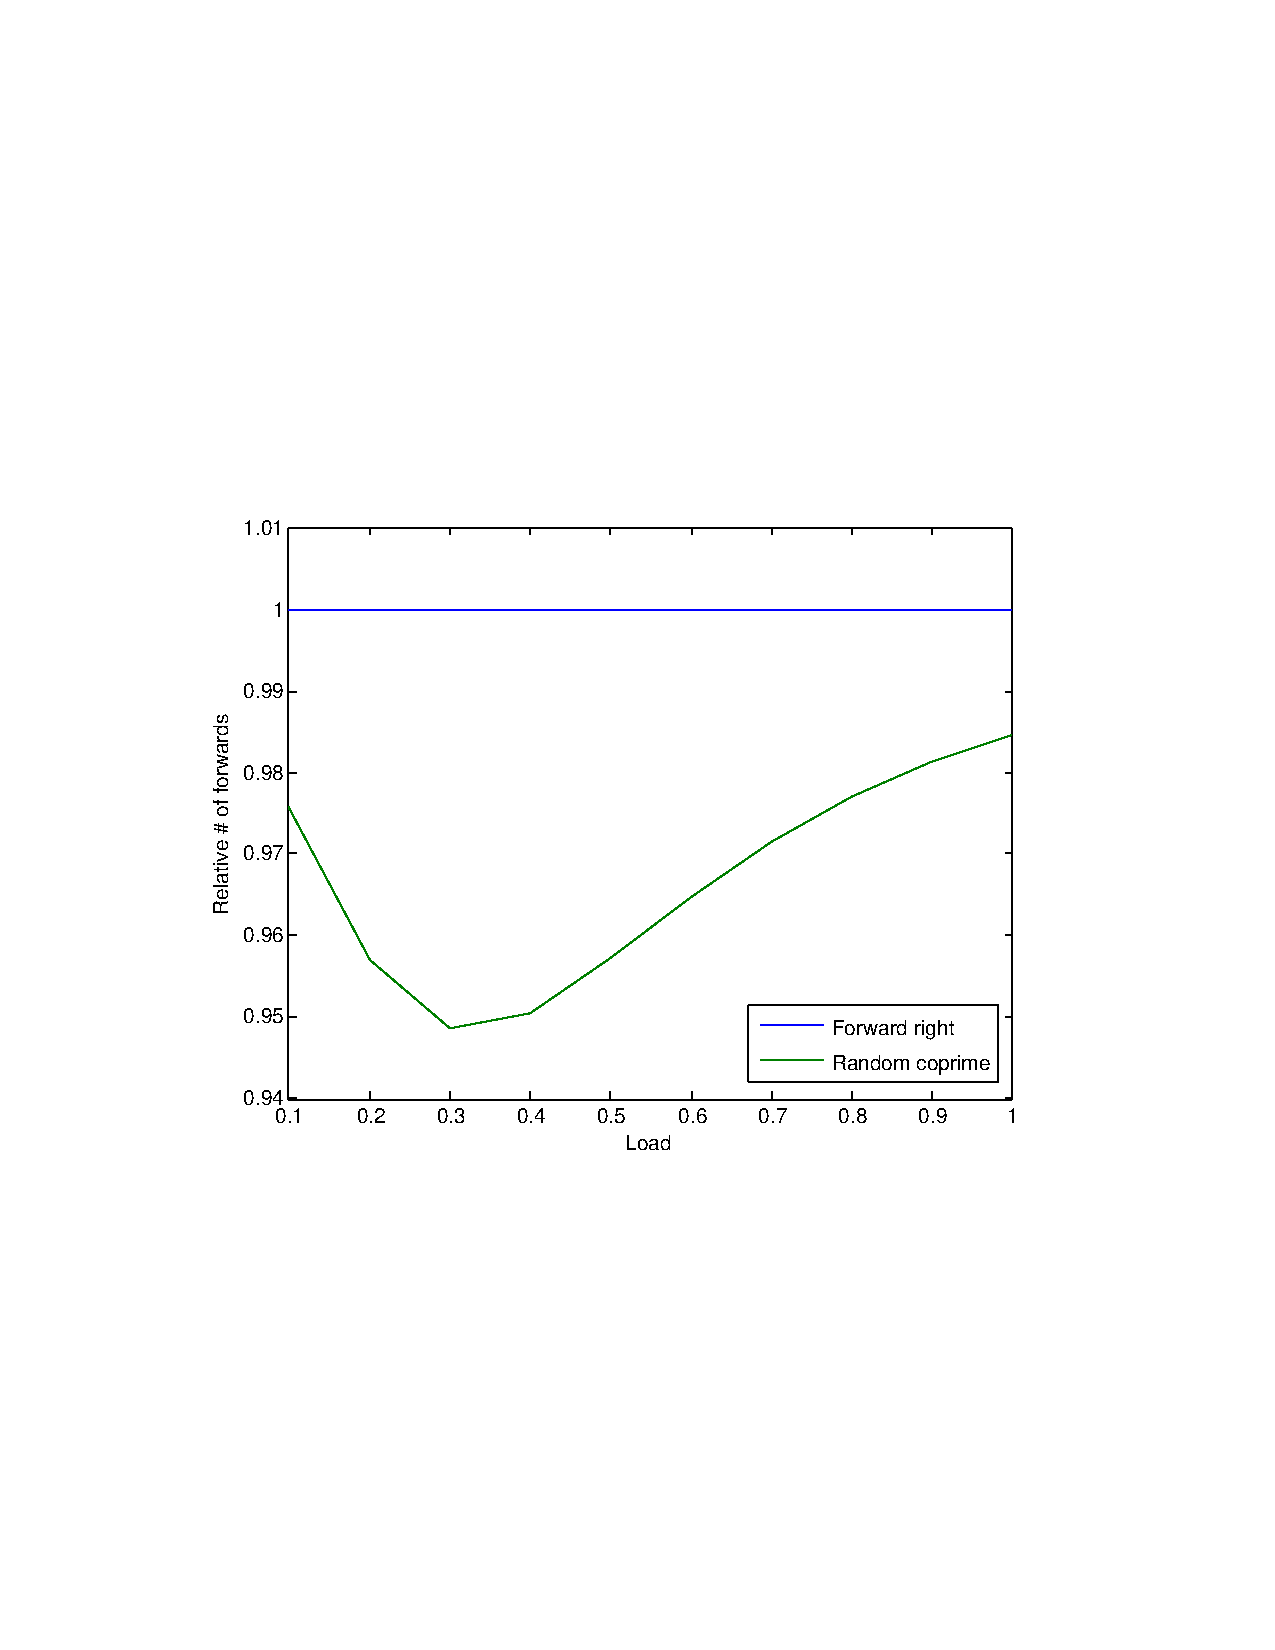
\includegraphics[clip=true, trim=9em 24em 9em 24em, width=0.9\textwidth]{resources/plotrandcoprime.pdf}
\caption{Validation of Coprime algorithm for $N=10$}
\label{validcp}
\end{figure}

As shown in figure \ref{validcp}, the performance gain of this algorithm is up to 5\% for a ring size of $N=10$. The list of coprimes in that scenario is ${1, 3, 7, 9}$, thus 4 possible choices. When increasing the ring size to $11$, a prime number, the list of coprimes expands to ${1..10}$ (because 11 is prime), thus 10 possible choices. This increases the relative performance gain up to 8\%. To make clear the increased performance is not due to the increase of $N$, figure \ref{validcp12} shows the performance gain for $N=12$.

\begin{figure}[h!tb]
\centering
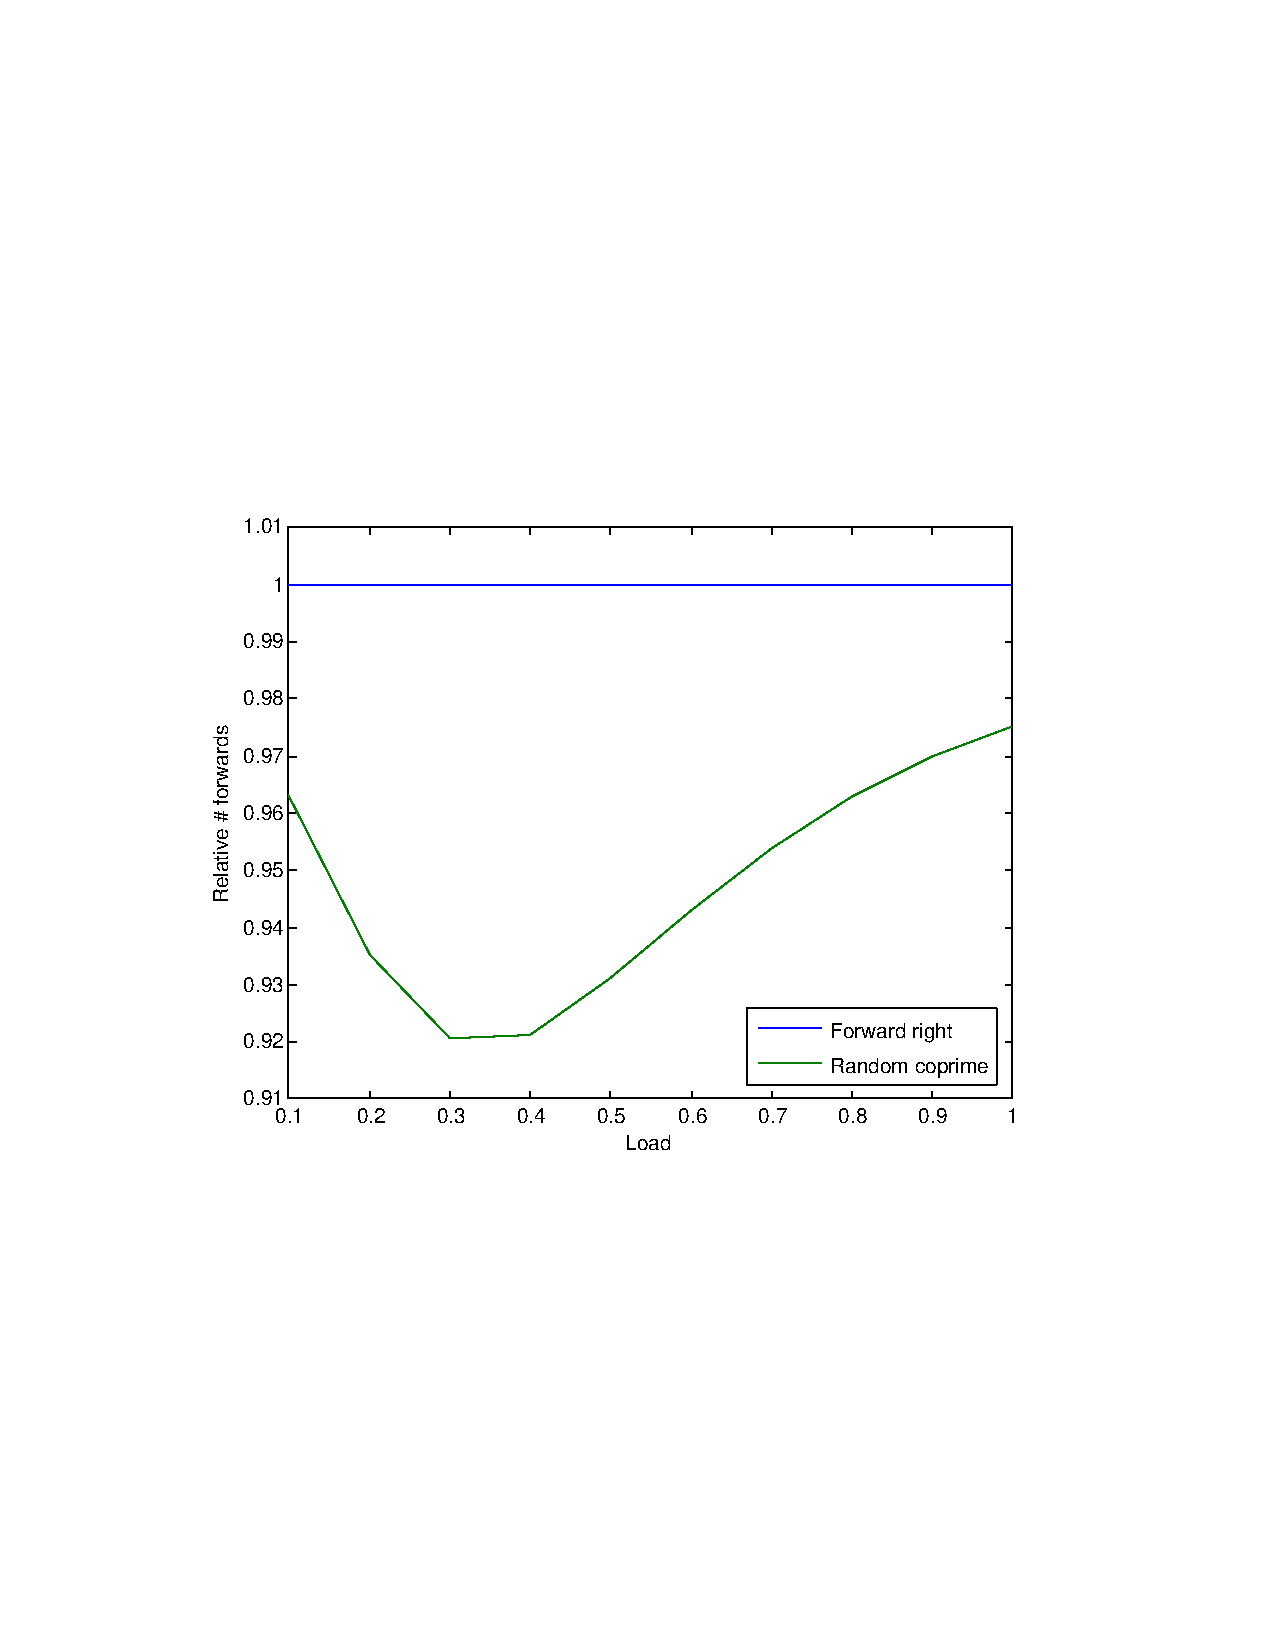
\includegraphics[clip=true, trim=9em 24em 9em 24em, width=0.9\textwidth]{resources/plotrandcoprime11.pdf}
\caption{Validation of Coprime algorithm for $N=11$}
\label{validcp11}
\end{figure}

\begin{figure}[h!tb]
\centering
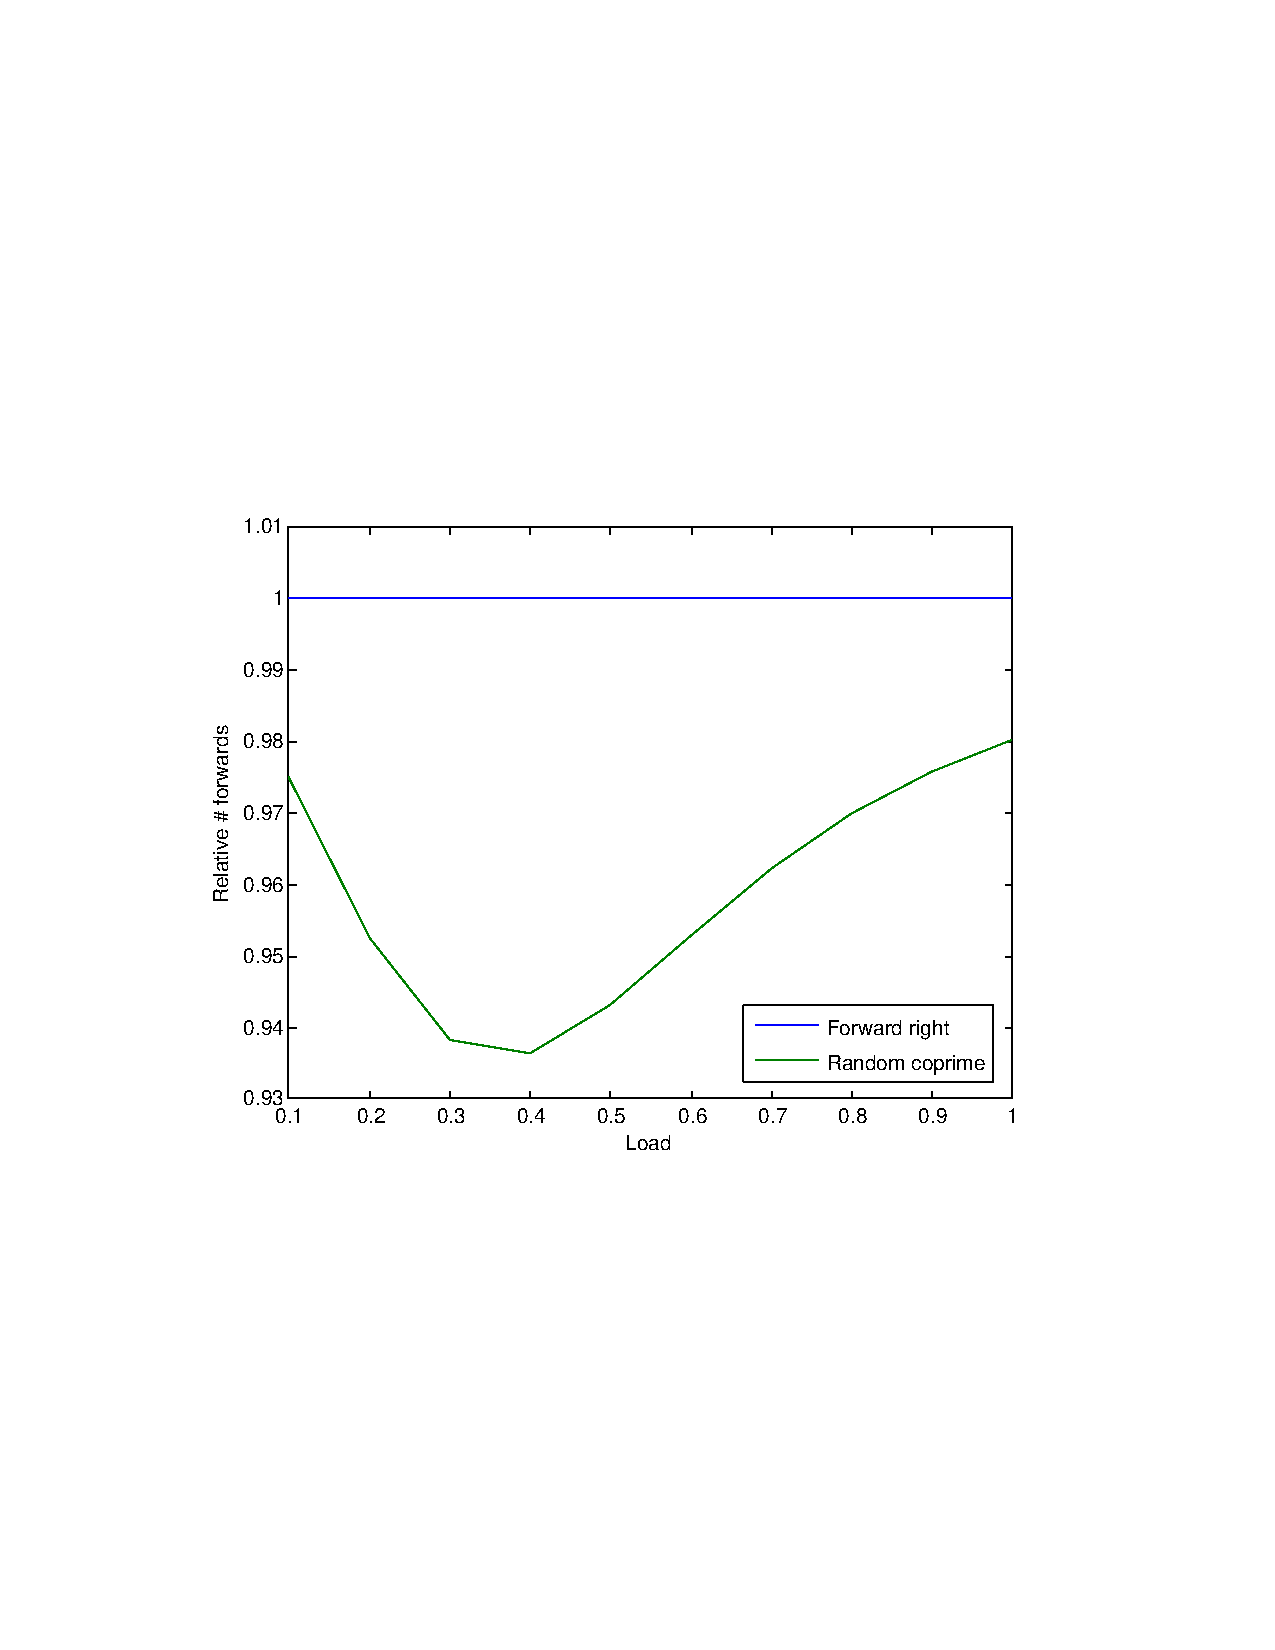
\includegraphics[clip=true, trim=9em 24em 9em 24em, width=0.9\textwidth]{resources/plotrandcoprime12.pdf}
\caption{Validation of Coprime algorithm for $N=12$}
\label{validcp12}
\end{figure}

The performance gain is dependant on the number of different paths a job can follow. For $N=10$ and $N=12$, a job can follow 4 possible routes, for $N=11$, 10 different routes can be chosen.


\subsection{Random Unvisited}
This problem can be modelled much more efficiently than the techniques. Since the next node is chosen at random, the information we need to save consists only of the number of servers which are currently busy. This problem is analogue to modelling an Erlang-B loss system. The number of states in this Markov Chain is linear to $N$, is much more dense and already represents a lumped Markov Chain. For $N=3$, the matrix is given below.

\[ Q =
  \begin{blockarray}{ccccc}
    & 0 & 1 & 2 & 3 \\
    \begin{block}{c[cccc]}
    0 & -3\lambda & 3\lambda & 0 & 0 \\
    1 & \mu & -3\lambda-\mu & 3\lambda & 0 \\
    2 & 0 & \mu & -3\lambda-\mu & 3\lambda \\
    3 & 0 & 0 & \mu & -\mu \\
    \end{block}
  \end{blockarray}
\]

\subsection{Lumped states}
\label{lump}

Except for Random Unvisited, each discribed technique is modelled into a Markov Chain with $N^2$ states. However, many of these states are redundant: for example, for $N=3$ the states $001$, $010$ and $100$ all represent one of the nodes being busy. For states representing multiple busy nodes, the space between these servers is critical information. Multiple states can be lumped when bitrotating one state can result in another state. Example: the states below are analogue and can therefore be lumped into one state:
\begin{verbatim}
001101 = 011010 = 110100 = 101001 = 010011 = 100110
\end{verbatim}

The example model in \ref{validateright} can be lumped into the following Markov Chain:

\[ Q =
  \begin{blockarray}{ccccc}
    & 000 & 001 & 011 & 111 \\
    \begin{block}{c[cccc]}
    000 & -3\lambda & 3\lambda & 0 & 0 \\
    001 & \mu & 3\lambda-\mu & 3\lambda & 0 \\
    011 & 0 & 2\mu & 3\lambda-2\mu & 3\lambda \\
    111 & 0 & 0 & 3\mu & -3\mu \\
    \end{block}
  \end{blockarray}
\]

Computing the steady state distribution of a Markov Chain is subject to time constraints. Using sparse matrices for our algorithm already solved the memory constraints.
Two factors are important when working with matrices: the number of elements and the number of nonzero elements. We will show that both factors are reduced significantly.

For unlumped Markov Chains modelling the Random forward algorithm, a matrix consists of $2^N$ states, an exponential growth. Lumping these matrices results in a number of states equal to:  $\frac{1}{N} \sum_{d|N} (2^{N/d} \cdot \phi(d) )$ where $\phi(d) = d \cdot \prod_{p|d, p\text{ is prime}} (1-\frac{1}{p})$ \cite{A000031}. Although this result greatly reduces the number of states, its complexity is still non-polynomial.

The number of nonzero elements for unlumped Markov Chains is $(N+1) 2^N$. For lumped matrices, we were not able to derive an exact formula, however, figure \ref{lumpnnz} shows a clear reduction as well. Yet, this result doesn't seem polynomial either.

\begin{figure}[h!tb]
\centering
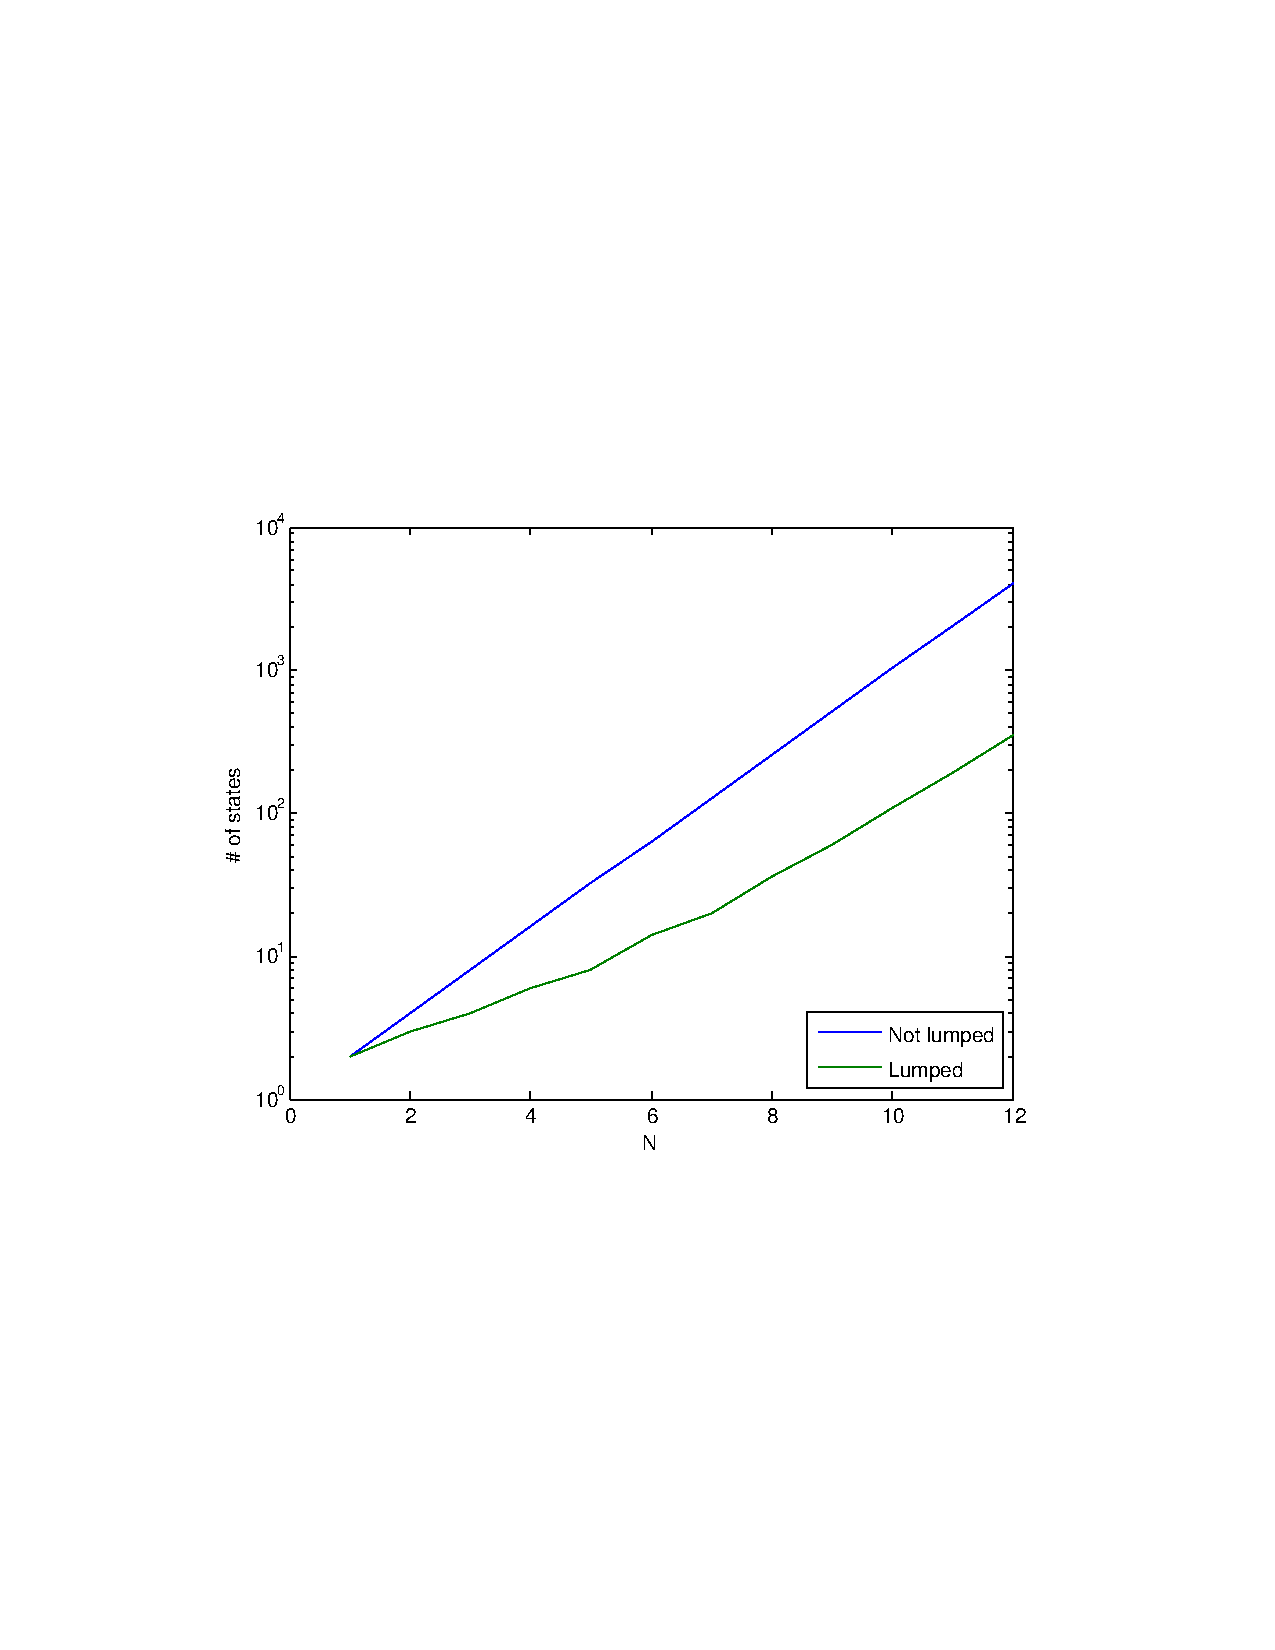
\includegraphics[clip=true, trim=9em 24em 9em 24em, width=0.9\textwidth]{resources/plotlumping.pdf}
\caption{Number of states}
\label{figlump}
\end{figure}

\begin{figure}[h!tb]
\centering
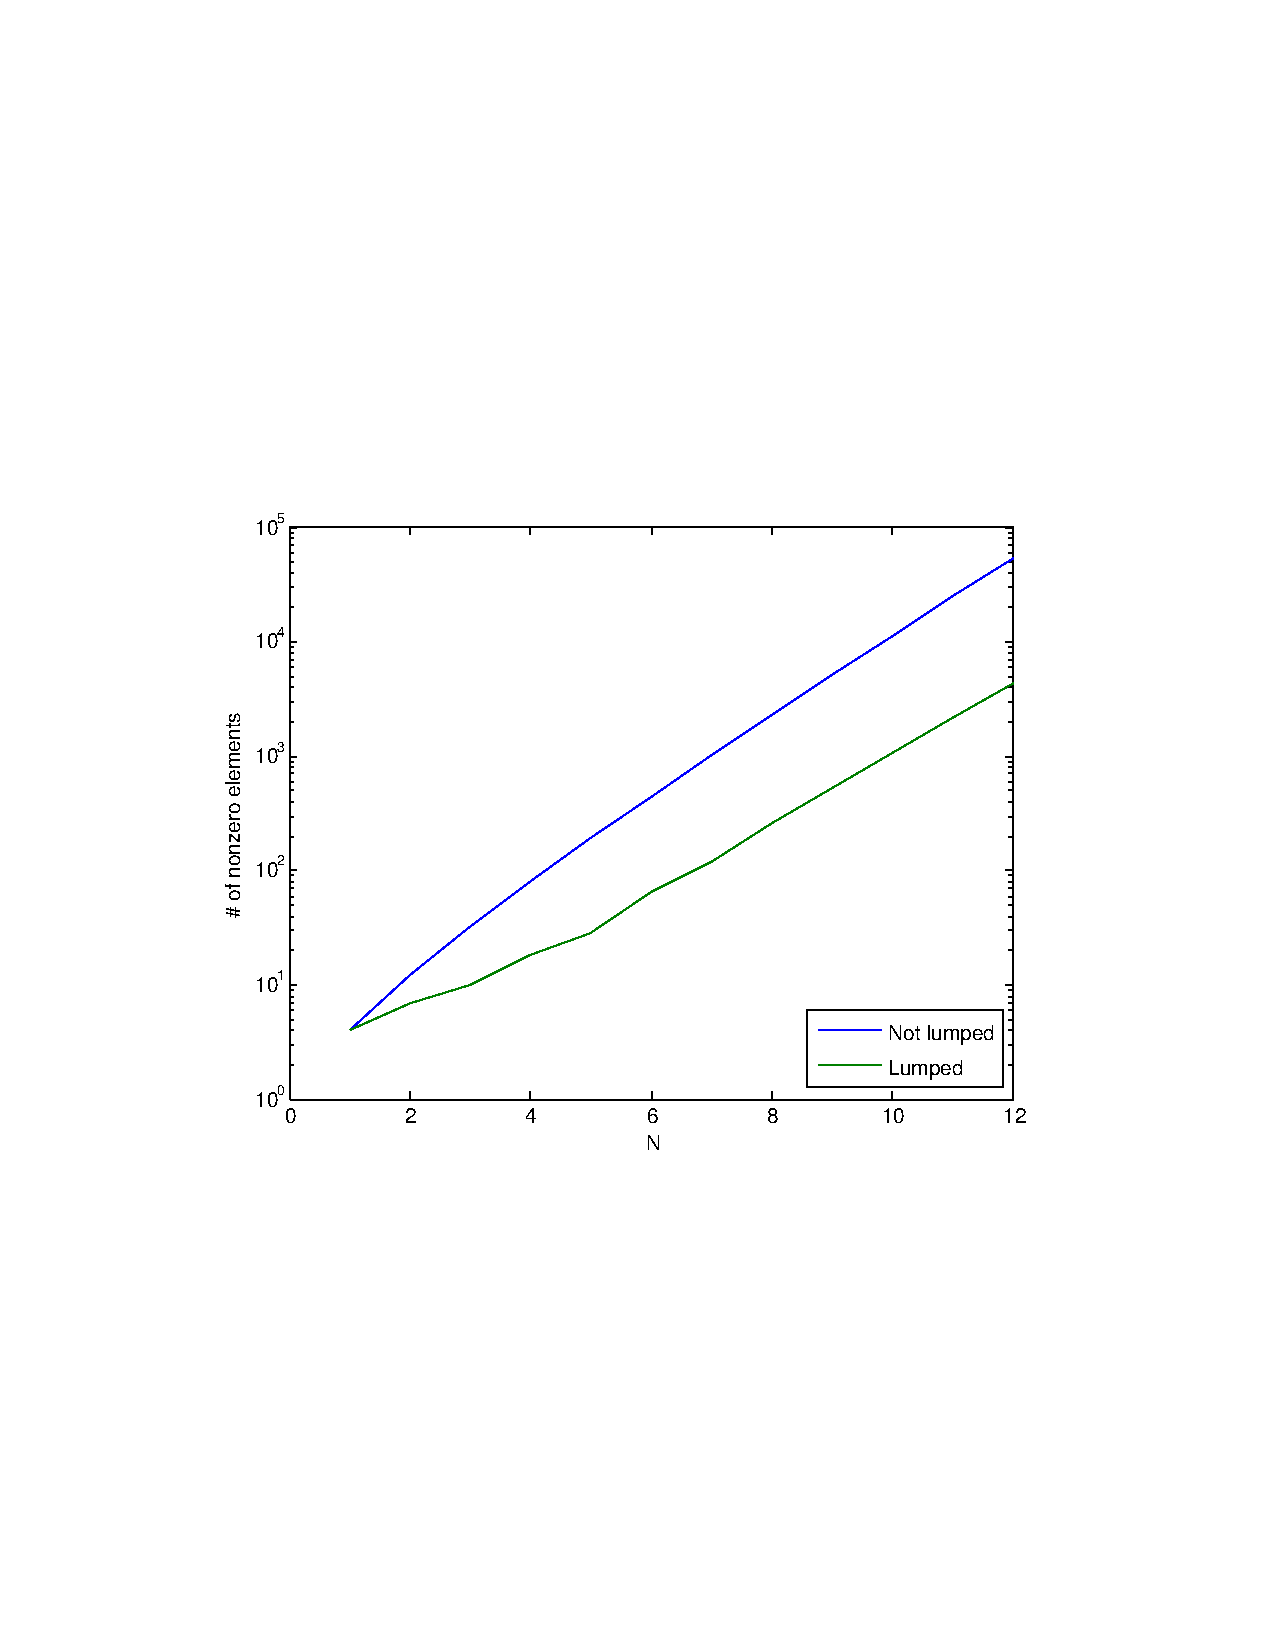
\includegraphics[clip=true, trim=9em 24em 9em 24em, width=0.9\textwidth]{resources/plotlumpingnnz.pdf}
\caption{Number of nonzero elements}
\label{lumpnnz}
\end{figure}

It seems lumping is a good technique to push the bounderies of the validation by reducing two important factors of the compution time. However, it is no silver bullet: both the number of states and the number of nonzero elements are nonpolynomial after lumping the matrices.

\subsection{Equivalent techniques}
Lumping states of a Markov Chain produces an equivalent Markov Chain. This can be used to prove some forwarding techniques are equal up to a certain $N$.

\section{Conclusion}
\label{secconclusion}

\begin{table}[h!]
\centering
\begin{tabular}{|p{0.25\textwidth}|p{0.25\textwidth}|p{0.25\textwidth}|p{0.25\textwidth}|} \hline
							& Max. gain		& Space requirement (bits)	& Notes \\ \hline
Forward Right				& 0 (baseline)	& 0							&		\\ \hline
Left/Right forward			& $> 4\%$		& 1 (job) + 1 (node)		&		\\ \hline
Random Left/Right forward	& 0 (worse)		& 1 (job)					&		\\ \hline
Position dependant forward	& 0 (worse)		& 1 (job)					& Creates loaded clusters \\ \hline
\end{tabular}
\caption{Forward to neighbor}
\end{table}

\begin{table}[h!]
\centering
\begin{tabular}{|p{0.4\textwidth}|p{0.3\textwidth}|p{0.3\textwidth}|} \hline
							& Max. gain		& Space requirement (bits)	\\ \hline
Random unvisited			& $> 24\%$		& $N$						\\ \hline
Coprime offset				& $> 24\%$		& $log_2 N$ (job) + $log_2 (\sum_{p < N,gcd(p, N) = 1} 1)$ (node) \\ \hline
Random Coprime offset		& $> 24\%$		& $log_2 N$					\\ \hline
\end{tabular}
\caption{Forward anywhere}
\end{table}


\begin{table}
\centering
\begin{tabular}{|p{0.4\textwidth}|p{0.3\textwidth}|p{0.25\textwidth}|p{0.3\textwidth}|} \hline
 							& Performance gain at load=0.5	& Number of possible paths	\\ \hline
Forward Right				& 0								& 1							\\ \hline
Left/Right forward			& $\approx 4.5\%$				& 2							\\ \hline
Random Left/Right (0.5)		& no gain						& 2							\\ \hline
Position-dependant forwarding & no gain						& 1							\\ \hline
Random unvisited			& $\approx 24\%$						& $(N-1)!$					\\ \hline
(Random) Coprime offset		& $\approx 24\%$						& $\sum_{p < N,gcd(p, N) = 1} 1$ \\ \hline
\end{tabular}
\caption{Performance gain vs number of paths}
\end{table}

Which techniques work best in which environments? Why? Runner up? Why do some techniques don't work as expected? performance results in function of number of paths

\printbibliography

\begin{changemargin}{-2cm}{-2cm}{4cm}

\appendix
\section{Simulator source code}
\label{sourcecode}

\lstset{tabsize=4,language=C++,caption={nodes.h}}
\lstinputlisting{../src/nodes.h}

\lstset{caption={servernode.cpp}}
\lstinputlisting{../src/servernode.cpp}

\lstset{caption={randswitchchain.m}}
\lstinputlisting{../src/configuration.h}

\lstset{caption={randswitchchain.m}}
\lstinputlisting{../src/nodes.cpp}

\lstset{caption={randswitchchain.m}}
\lstinputlisting{../src/Main.cpp}

\lstset{caption={randswitchchain.m}}
\lstinputlisting{../src/servernode.h}

\lstset{caption={randswitchchain.m}}
\lstinputlisting{../src/ring/ring.cpp}

\lstset{caption={randswitchchain.m}}
\lstinputlisting{../src/ring/job.h}

\lstset{caption={randswitchchain.m}}
\lstinputlisting{../src/ring/node.h}

\lstset{caption={randswitchchain.m}}
\lstinputlisting{../src/ring/ring.h}

\lstset{caption={randswitchchain.m}}
\lstinputlisting{../src/ring/node.cpp}

\lstset{caption={randswitchchain.m}}
\lstinputlisting{../src/ring/arriveevent.h}

\lstset{caption={randswitchchain.m}}
\lstinputlisting{../src/ring/job.cpp}

\lstset{caption={randswitchchain.m}}
\lstinputlisting{../src/ring/finishevent.h}

\lstset{caption={randswitchchain.m}}
\lstinputlisting{../src/configuration.cpp}

\lstset{caption={randswitchchain.m}}
\lstinputlisting{../src/simulator/schedule.h}

\lstset{caption={randswitchchain.m}}
\lstinputlisting{../src/simulator/event.h}

\lstset{caption={randswitchchain.m}}
\lstinputlisting{../src/simulator/simulator.h}

\lstset{caption={randswitchchain.m}}
\lstinputlisting{../src/simulator/simulator.cpp}

\lstset{caption={randswitchchain.m}}
\lstinputlisting{../src/simulator/schedule.cpp}

\section{MATLAB Numerical evaluation code}
\label{matlabcode}

\lstset{tabsize=8,language=Octave,caption={rightchain.m}}
\lstinputlisting{../matlab/rightchain.m}

\lstset{caption={randswitchchain.m}}
\lstinputlisting{../matlab/randswitchchain.m}

\lstset{caption={rprimechain.m}}
\lstinputlisting{../matlab/rprimechain.m}

\lstset{caption={runvisitedchain.m}}
\lstinputlisting{../matlab/runvisitedchain.m}

\lstset{caption={avghops.m}}
\lstinputlisting{../matlab/avghops.m}

\lstset{caption={ruavghops.m}}
\lstinputlisting{../matlab/ruavghops.m}

\lstset{caption={ctmcsteadystate.m}}
\lstinputlisting{../matlab/ctmcsteadystate.m}

\lstset{caption={lumpavghops.m}}
\lstinputlisting{../matlab/lumpavghops.m}

\lstset{caption={lump.m}}
\lstinputlisting{../matlab/lump.m}

\lstset{caption={makestates.m}}
\lstinputlisting{../matlab/makestates.m}

\end{changemargin}

\end{document}